%%%%%%%%%%%%%%%%%%%%%%%%%%%%%%%%%%%%%%%%
% datoteka.tex
%



\documentclass[a4paper, 12pt]{book}
%\documentclass[a4paper, 12pt, draft]{book}  Nalogo preverite tudi z opcijo draft, ki vam bo pokazala, katere vrstice so predolge!


\usepackage{float}
\usepackage[utf8x]{inputenc}   % omogoča uporabo slovenskih črk kodiranih v formatu UTF-8
\usepackage[slovene,english]{babel}    % naloži, med drugim, slovenske delilne vzorce
\usepackage[pdftex]{graphicx}  % omogoča vlaganje slik različnih formatov
\usepackage{fancyhdr}          % poskrbi, na primer, za glave strani
\usepackage{amssymb}           % dodatni simboli
\usepackage{amsmath}           % eqref, npr.
%\usepackage{hyperxmp}
\usepackage[hyphens]{url}  % dodal Solina
\usepackage{comment}       % dodal Solina

\usepackage[pdftex, colorlinks=true,
						citecolor=black, filecolor=black, 
						linkcolor=black, urlcolor=black,
						pagebackref=false, 
						pdfproducer={LaTeX}, pdfcreator={LaTeX}, hidelinks]{hyperref}

\usepackage{color}       % dodal Solina
\usepackage{soul}       % dodal Solina


%%%%%%%%%%%%%%%%%%%%%%%%%%%%%%%%%%%%%%%%
%	CUSTOME
%%%%%%%%%%%%%%%%%%%%%%%%%%%%%%%%%%%%%%%%
\usepackage{array}
\usepackage{tabularx}
\usepackage{listings}
\usepackage{xcolor}


\renewcommand{\lstlistingname}{Koda}
\renewcommand{\lstlistlistingname}{Seznam kod}

\newcolumntype{b}{X}
\newcolumntype{s}{>{\hsize=.9\hsize}X}
\newcolumntype{z}{>{\hsize=.2\hsize}X}

\definecolor{codegreen}{rgb}{0,0.6,0}
\definecolor{codegray}{rgb}{0.5,0.5,0.5}
\definecolor{codepurple}{rgb}{0.20,0,0.82}
\definecolor{backcolour}{rgb}{0.97,0.97,0.97}

\lstdefinestyle{mystyle}{
    backgroundcolor=\color{backcolour},   
    commentstyle=\color{codegreen},
    keywordstyle=\color{magenta},
    numberstyle=\tiny\color{codegray},
    stringstyle=\color{codepurple},
    basicstyle=\ttfamily\footnotesize,
    breakatwhitespace=false,         
    breaklines=true,                 
    captionpos=b,                    
    keepspaces=true,                 
    numbers=left,                    
    numbersep=5pt,                  
    showspaces=false,                
    showstringspaces=false,
    showtabs=false,                  
    tabsize=2
}

%%%%%%%%%%%%%%%%%%%%%%%%%%%%%%%%%%%%%%%%
%	DIPLOMA INFO
%%%%%%%%%%%%%%%%%%%%%%%%%%%%%%%%%%%%%%%%
\newcommand{\ttitle}{Spletni portal - Urejanje in pregled raziskovalnih objav s področja hrane}
\newcommand{\ttitleEn}{Web Portal -  Reviewing and managing publications of food research }
\newcommand{\tsubject}{\ttitle}
\newcommand{\tsubjectEn}{\ttitleEn}
\newcommand{\tauthor}{Žiga Marolt}
\newcommand{\tkeywords}{spletna aplikcija, Go, Vue.js, mikrostoritev, vsebniki, Docker, spletni strežnik, OpenApi, HTTP, TLS, PostgreSQL, Tailwind, CSS, HTML, CQRS}
\newcommand{\tkeywordsEn}{web application, Go, Vue.js, microservice, containers, Docker, web server, OpenApi, TLS, HTTP, TLS, PostgreSQL, Tailwind, CSS, HTML, CQRS}


%%%%%%%%%%%%%%%%%%%%%%%%%%%%%%%%%%%%%%%%
%	HYPERREF SETUP
%%%%%%%%%%%%%%%%%%%%%%%%%%%%%%%%%%%%%%%%
\hypersetup{pdftitle={\ttitle}}
\hypersetup{pdfsubject=\ttitleEn}
\hypersetup{pdfauthor={\tauthor, zm1218@student.uni-lj.si}}
\hypersetup{pdfkeywords=\tkeywordsEn}


%%%%%%%%%%%%%%%%%%%%%%%%%%%%%%%%%%%%%%%%
% postavitev strani
%%%%%%%%%%%%%%%%%%%%%%%%%%%%%%%%%%%%%%%%  

\addtolength{\marginparwidth}{-20pt} % robovi za tisk
\addtolength{\oddsidemargin}{40pt}
\addtolength{\evensidemargin}{-40pt}

\renewcommand{\baselinestretch}{1.3} % ustrezen razmik med vrsticami
\setlength{\headheight}{15pt}        % potreben prostor na vrhu
\renewcommand{\chaptermark}[1]%
{\markboth{\MakeUppercase{\thechapter.\ #1}}{}} \renewcommand{\sectionmark}[1]%
{\markright{\MakeUppercase{\thesection.\ #1}}} \renewcommand{\headrulewidth}{0.5pt} \renewcommand{\footrulewidth}{0pt}
\fancyhf{}
\fancyhead[LE,RO]{\sl \thepage} 
\fancyhead[LO]{\sl \rightmark} \fancyhead[RE]{\sl \leftmark}
% \fancyhead[RE]{\sc \tauthor}              % dodal Solina
% \fancyhead[LO]{\sc Diplomska naloga}     % dodal Solina


\newcommand{\BibTeX}{{\sc Bib}\TeX}

%%%%%%%%%%%%%%%%%%%%%%%%%%%%%%%%%%%%%%%%
% naslovi
%%%%%%%%%%%%%%%%%%%%%%%%%%%%%%%%%%%%%%%%  


\newcommand{\autfont}{\Large}
\newcommand{\titfont}{\LARGE\bf}
\newcommand{\clearemptydoublepage}{\newpage{\pagestyle{empty}\cleardoublepage}}
\setcounter{tocdepth}{1}	      % globina kazala

%%%%%%%%%%%%%%%%%%%%%%%%%%%%%%%%%%%%%%%%
% konstrukti
%%%%%%%%%%%%%%%%%%%%%%%%%%%%%%%%%%%%%%%%  
\newtheorem{izrek}{Izrek}[chapter]
\newtheorem{trditev}{Trditev}[izrek]
\newenvironment{dokaz}{\emph{Dokaz.}\ }{\hspace{\fill}{$\Box$}}

%%%%%%%%%%%%%%%%%%%%%%%%%%%%%%%%%%%%%%%%%%%%%%%%%%%%%%%%%%%%%%%%%%%%%%%%%%%%%%%
%% PDF-A
%%%%%%%%%%%%%%%%%%%%%%%%%%%%%%%%%%%%%%%%%%%%%%%%%%%%%%%%%%%%%%%%%%%%%%%%%%%%%%%


%%%%%%%%%%%%%%%%%%%%%%%%%%%%%%%%%%%%%%%% 
% define medatata
%%%%%%%%%%%%%%%%%%%%%%%%%%%%%%%%%%%%%%%% 
\def\Title{\ttitle}
\def\Author{\tauthor, zm1218@student.uni-lj.si}
\def\Subject{\ttitleEn}
\def\Keywords{\tkeywordsEn}

%%%%%%%%%%%%%%%%%%%%%%%%%%%%%%%%%%%%%%%% 
% \convertDate converts D:20080419103507+02'00' to 2008-04-19T10:35:07+02:00
%%%%%%%%%%%%%%%%%%%%%%%%%%%%%%%%%%%%%%%% 
\def\convertDate{%
    \getYear
}

{\catcode`\D=12
 \gdef\getYear D:#1#2#3#4{\edef\xYear{#1#2#3#4}\getMonth}
}
\def\getMonth#1#2{\edef\xMonth{#1#2}\getDay}
\def\getDay#1#2{\edef\xDay{#1#2}\getHour}
\def\getHour#1#2{\edef\xHour{#1#2}\getMin}
\def\getMin#1#2{\edef\xMin{#1#2}\getSec}
\def\getSec#1#2{\edef\xSec{#1#2}\getTZh}
\def\getTZh +#1#2{\edef\xTZh{#1#2}\getTZm}
\def\getTZm '#1#2'{%
    \edef\xTZm{#1#2}%
    \edef\convDate{\xYear-\xMonth-\xDay T\xHour:\xMin:\xSec+\xTZh:\xTZm}%
}

\expandafter\convertDate\pdfcreationdate 

%%%%%%%%%%%%%%%%%%%%%%%%%%%%%%%%%%%%%%%%
% get pdftex version string
%%%%%%%%%%%%%%%%%%%%%%%%%%%%%%%%%%%%%%%% 
\newcount\countA
\countA=\pdftexversion
\advance \countA by -100
\def\pdftexVersionStr{pdfTeX-1.\the\countA.\pdftexrevision}


%%%%%%%%%%%%%%%%%%%%%%%%%%%%%%%%%%%%%%%%
% XMP data
%%%%%%%%%%%%%%%%%%%%%%%%%%%%%%%%%%%%%%%%  
\usepackage{xmpincl}

%%%%%%%%%%%%%%%%%%%%%%%%%%%%%%%%%%%%%%%%
% pdfInfo
%%%%%%%%%%%%%%%%%%%%%%%%%%%%%%%%%%%%%%%%  
\pdfinfo{%
    /Title    (\ttitle)
    /Author   (\tauthor, zm1218@student.uni-lj.si)
    /Subject  (\ttitleEn)
    /Keywords (\tkeywordsEn)
    /ModDate  (\pdfcreationdate)
    /Trapped  /False
}

% list

\newenvironment{myitemize}
{ \begin{itemize}
    \setlength{\itemsep}{2pt}
    \setlength{\parskip}{0pt}
    \setlength{\parsep}{2pt}     }
{ \end{itemize}                  } 


%%%%%%%%%%%%%%%%%%%%%%%%%%%%%%%%%%%%%%%%%%%%%%%%%%%%%%%%%%%%%%%%%%%%%%%%%%%%%%%
%%%%%%%%%%%%%%%%%%%%%%%%%%%%%%%%%%%%%%%%%%%%%%%%%%%%%%%%%%%%%%%%%%%%%%%%%%%%%%%
\begin{document}
\selectlanguage{slovene}
\frontmatter
\setcounter{page}{1} %
\renewcommand{\thepage}{}       % preprecimo težave s številkami strani v kazalu
\newcommand{\sn}[1]{"`#1"'}                    % dodal Solina (slovenski narekovaji)

%%%%%%%%%%%%%%%%%%%%%%%%%%%%%%%%%%%%%%%%
%naslovnica
 \thispagestyle{empty}%
   \begin{center}
    {\large\sc Univerza v Ljubljani\\%
      Fakulteta za računalništvo in informatiko}%
    \vskip 10em%
    {\autfont \tauthor\par}%
    {\titfont \ttitle \par}%
    {\vskip 3em \textsc{DIPLOMSKO DELO\\[5mm]       
    VISOKOŠOLSKI STROKOVNI ŠTUDIJSKI PROGRAM\\ PRVE STOPNJE\\ RAČUNALNIŠTVO IN INFORMATIKA}\par}%
    \vfill\null%
    {\large \textsc{Mentor}: doc.\ dr.  Mira Trebar\par}%
    {\vskip 2em \large Ljubljana, 2021 \par}%
\end{center}
% prazna stran
%\clearemptydoublepage      % dodal Solina (izjava o licencah itd. se izpiše na hrbtni strani naslovnice)

%%%%%%%%%%%%%%%%%%%%%%%%%%%%%%%%%%%%%%%%
%copyright stran
\thispagestyle{empty}
\vspace*{8cm}

\noindent
{\sc Copyright}. 
Rezultati diplomske naloge so intelektualna lastnina avtorja in Fakultete za računalništvo in informatiko Univerze v Ljubljani.
Za objavo in koriščenje rezultatov diplomske naloge je potrebno pisno privoljenje avtorja, Fakultete za računalništvo in informatiko ter mentorja.

\begin{center}
\mbox{}\vfill
\emph{Besedilo je oblikovano z urejevalnikom besedil \LaTeX.}
\end{center}
% prazna stran
\clearemptydoublepage

%%%%%%%%%%%%%%%%%%%%%%%%%%%%%%%%%%%%%%%%
% stran 3 med uvodnimi listi
\thispagestyle{empty}
\vspace*{4cm}

\noindent
Fakulteta za računalništvo in informatiko izdaja naslednjo nalogo:
\medskip
\begin{tabbing}
\hspace{32mm}\= \hspace{6cm} \= \kill




Tematika naloge:
\end{tabbing}

Spletna aplikacija za pregled raziskovalnih metod s področja analize in napovedovanja dobe uporabnosti hitro pokvarljivih živil, kot sta sveže meso in ribe. V aplikaciji se uporablja pristop vodenja evidenc.  Ta metoda kot vir podatkov uporablja že obstoječe zanesljive dokumente in podobne vire informacij za zbiranje podatkov. Na osnovi vnaprej definiranih živil se za izbrano živilo nahajajo podatki, ki omogočajo pregled zahtev v hladni verigi, raziskovalnih metod, raziskovalcev, inštitucij, raziskovalnih laboratorijev, objavljenih člankov, podatkovnih baz, programskih orodij, …

Obseg naloge in podrobnejši opis bi definirali v nadaljevanju. Pomembno je, da bi zasnovali ustrezen
model podatkovne baze tako, da lahko v aplikaciji  prijavljen uporabnik dodaja vsebine za neko živilo.
Pred objavo, pa jih mora potrditi odgovorna oseba. Zasnovana mora biti tako, da je možno do nje
dostopati iz poljubne aplikacije. Testiranje bi izvedli z enostavnim spletnim portalom, kjer bi vnesli
testne podatke iz nekaj raziskovalnih člankov.

\vspace{15mm}






\vspace{2cm}

% prazna stran
\clearemptydoublepage

% zahvala
\thispagestyle{empty}\mbox{}\vfill\null\it%
\noindent
Zahvaljujem se mentorici doc. dr. Miri Trebar za vso pomoč in družini za podporo.
\rm\normalfont

% prazna stran
\clearemptydoublepage


%%%%%%%%%%%%%%%%%%%%%%%%%%%%%%%%%%%%%%%%
% kazalo
\pagestyle{empty}
\def\thepage{}% preprecimo tezave s stevilkami strani v kazalu
\tableofcontents{}


% tole naj bi mi kao clearalo empty page pa mi ne !
\let\cleardoublepage=\clearpage

%%%%%%%%%%%%%%%%%%%%%%%%%%%%%%%%%%%%%%%%
% seznam kratic

\chapter*{Seznam uporabljenih kratic}  % spremenil Solina, da predolge vrstice ne gredo preko desnega roba
\noindent\begin{tabular}{p{0.2\textwidth}|p{.35\textwidth}|p{.35\textwidth}}    % po potrebi razširi prvo kolono tabele na račun drugih dveh!
  {\bf kratica} & {\bf angleško}                             & {\bf slovensko} \\ \hline
  {\bf API} & Application Programming Interface & aplikacijski programski vmesnik \\
  {\bf IAAA} & Identification, Authentication, Authorization and Accounting & varnostni koncepti: identifikacija, avtentikacija, avtorizacija in odgovornost \\
  {\bf CSS} & Cascading Style Sheets & predloge, ki določajo izgled spletnih strani \\
  {\bf ER diagram} & Entity Relationship Diagram & entitetno relacijski diagram \\
  {\bf HTML} & Hyper Text Markup Language & označevalni jezik za izdelavo spletnih strani \\
  {\bf HTTP} & Hyper Text Transfer Protocol & komunikacijski spletni protokol \\
  {\bf JSON} & JavaScript Object Notation & objektna notacija za JavaScript \\
  {\bf oktet} byte & Digitalna enota, ki predstavlja osem bitov \\
%   {\bf PDF} & Portable Document Format & format prenosnega dokumenta \\
  {\bf REST} & Representational state transfer & predstavitveni prenos stanja \\
  {\bf SQL} & Structured Query Language & strukturiran poizvedovalni jezik \\
  {\bf URL} & Uniform Resource Locator & enolični krajevnik vira \\
%  \dots & \dots & \dots \\
\end{tabular}


% prazna stran
\clearemptydoublepage

%%%%%%%%%%%%%%%%%%%%%%%%%%%%%%%%%%%%%%%%
% povzetek
\addcontentsline{toc}{chapter}{Povzetek}
\chapter*{Povzetek}

\noindent\textbf{Naslov:} \ttitle
\bigskip

\noindent\textbf{Avtor:} \tauthor
\bigskip

%\noindent\textbf{Povzetek:} 
\noindent
Dandanes se na spletu pojavlja vedno več raziskovalnih metod iz področja analize in napovedovanja dobe uporabnosti hitro pokvarljivih živil, kot sta naprimer sveže meso in ribe. Vsaka raziskovalna metoda lahko pri raziskovanju uporablja različne parametre. Parametri se razlikujejo glede na format, strukturo ali pa samo vrsto podatkov. 

Namen te diplomske naloge je izdelati spletno aplikacijo, s primerno podatkovno shemo. Preko nje je mogoče dodajati, urejati, brisati in iskati po vnesenih raziskovalnih metodah. Dostop do posameznih delov aplikacije je dovoljen le določenim uporabnikom, z ustreznimi uporabniškimi pravicami. Vpeljali bomo sistem avtentikacije in avtorizacije.

Skozi diplomsko nalogo bomo opisali celoten proces izdelovanja naše aplikacije, zasnovano z kot mikrostoritev v programskem jeziku Go. Spoznali bomo na kaj vse je potrebno biti pozoren pri zasnovi arhitekture spletne aplikacije, iz vidika varnosti podatkov, hitrosti razvoja aplikacije in hitrosti same aplikacije. Na koncu pa bomo spoznali še samo uporabo in uporabniško izkušnjo z primerom uporabe testnih podatkov.
\bigskip

\noindent\textbf{Ključne besede:} \tkeywords.
% prazna stran
\clearemptydoublepage

%%%%%%%%%%%%%%%%%%%%%%%%%%%%%%%%%%%%%%%%
% abstract
\selectlanguage{english}
\addcontentsline{toc}{chapter}{Abstract}
\chapter*{Abstract}

\noindent\textbf{Title:} \ttitleEn
\bigskip

\noindent\textbf{Author:} \tauthor
\bigskip

%\noindent\textbf{Abstract:} 
\noindent
Uvod v anglescini
\bigskip

\noindent\textbf{Keywords:} \tkeywordsEn.
\selectlanguage{slovene}
% prazna stran
\clearemptydoublepage

%%%%%%%%%%%%%%%%%%%%%%%%%%%%%%%%%%%%%%%%
\mainmatter
\setcounter{page}{1}
\pagestyle{fancy}

\chapter{Uvod}

Rok uporabnosti živila je pomembna oznaka vsakega živila. Podaja nam informacijo, koliko časa lahko neko živilo hranimo, da varnost in kakovost izdelka ostaneta v sprejemljivem območju. Ob tem morajo biti upoštevani specifični pogoji transporta in shranjevanja. Določitev roka uporabnosti živila temelji na predpostavki, da z živilom ustrezno ravnamo.

Iz dneva v dan nam je na voljo vedno več objavljenih raziskav iz področja hrane. Raziskave so objavljene na različnih virih, naj si bo to članek na svetovnem spletu, v reviji ali pa v znanstveni knjigi. Raziskovalci, ki prebirajo raziskave, imajo oteženo delo, poiskati zanesljive vire in iz njih izluščiti pravilne in informativne informacije.

V diplomski nalogi je opisan postopek izdelave spletne aplikacije za vnašanje in pregled raziskovalnih publikacij s področja analize in napovedovanja dobe uporabnosti hitro pokvarljivih živil. Aplikacija je zasnovana kot mikrostoritev. Za razvojno okolje je uporabljena docker arhitektura, kar nam omogoča enostavno postavitev projekta, in pa tudi enostavno objavljanje projekta na pravem okolju. 

Ker se struktura podatkov razlikuje od raziskave do reziskave, od vira do vira, je pomembno da pravilno definiramo podatkovno strukturo. Za dobro uporabniško izkušnjo mora biti vnos podatkov o raziskavah enostaven in dosleden, iskanje po le teh pa mora biti hitro in uporabno. Definirali smo več vrst uporabnikov, ki imajo različne dostope do posameznih delov aplikacije.

Med razvojem te aplikacije, ki vam jo bom opisal skozi celotno delo, sem se hotel naučiti čim več. Spoznal sem nov programski jezik - \verb=Go= in nov arhitekturni koncept mikro storitev (angl. microservice). Omenjeni dve stvari sta me dodatno spodbudili k delu in spoznavanju novih stvari na področju razvoja programske opreme in pa tudi same organizacije dela.

Skozi diplomsko nalogo bomo spoznali, najprej kako smo pristopili k reševanju omenjenega problema, kakšen je bil proces dela in sam razvoj aplikacije. Na koncu bomo spoznali še končno rešitev in samo implementacijo.


% \section{Motivacija}


% Priznajmo si, večina spletnih aplikacij ne rešuje težkih tehničnih izzivov. Pomembno je, da z izdelkom pridemo na trg pred našo konkurenco, zato pa je pomembno, da je izdelek pravilno tehnično strukturiran.
% Morda se to sprva sliši dolgočasno, vendar sam mislim, da je podpirati ta cilj težje, kot se sliši.




\chapter{Pregled področja}
\label{pregled-podrocja}
Varno uživanje živil zagotavljamo, če upoštevamo rok uporabnosti, poznamo in upoštevamo navodila proizvajalcev za shranjevanje živil, pri hitro pokvarljivih živilih pa vzdržujemo hladno verigo od proizvajalca do končnega uporabnika. Tako zmanjšujemo verjetnost nastanka okužb in zastrupitev, povzročenih z živili, nenazadnje pa tudi na količine živilskih odpadkov.

Zamrzovanje živil je eden izmed načinov podaljševanja roka uporabnosti živil. Zamrzniti je mogoče skoraj vsa živila z redkimi izjemami, vendar se je treba zavedati, da kakovost vseh živil po zamrzovanju ni enaka.

\textbf{Hladna veriga} je vzdrževanje predpisane, dovolj nizke, temperature živila, s ciljem ohranitve čim boljše kakovosti in varnosti živila v celotni živilski verigi, od proizvodnje, transporta, 
shranjevanja in distribucije do porabe pri končnem potrošniku. 
Običajno je to temperatura 4−8 °C, pri kateri se razvoj mikroorganizmov upočasni. Priporočena temperatura je predpisana na označbi izdelka. \cite{nijz-brosura-varnost}

V tabeli spodaj \ref{tab:food-safety-table} navajamo orientacijske vrednosti okvirnega roka uporabnosti takega živila.

\begin{table}[h]
\begin{tabular}{lll}
\textbf{Predelano živilo} & \textbf{Neodprto, po nakupu} & \textbf{Po odprtju}        \\
Kuhana perutnina          & 3 do 4 dni                   & 3 do 4 dni                 \\
Kuhane klobase            & 3 do 4 dni                   & 3 do 4 dni                 \\
Dimljene klobase          & 6 tednov/shramba             & 3 tedne                    \\
Slanina                   & 2 tedna                      & 7 dni                      \\
Hrenovke                  & 2 tedna                      & 1 teden                    \\
Šunka, kuhana             & 7 dni                        & rezine 3 dni; v kosu,7 dni
\end{tabular}
\caption{ Povzeto po USDA, Food safety and inspection service, 2011 }
\label{tab:food-safety-table}
\end{table}

\section{Pregled zahtev}

Namen aplikacije je, agregirati podatke iz različnih virov. Naj bo to knjiga, spletni vir ali pa revija. Vnašanje le teh podatkov iz nedefiniranih virov je težko in zamudno opravilo. Aplikacija mora biti razvita z namenom, da je uporabniku delo olajšano, z v naprej predlaganimi vrednostmi za posamezne podatke. 

Pomembno je, da zasnujemo ustrezen model podatkovne baze tako, da lahko v aplikaciji prijavljen uporabnik dodaja in ureja vsebine za neko živilo ne glede na to iz katerega vira izhajajo podatki. 
Struktura podatkov je lahko različna glede na vire podatkov, zatorej je potrebno razmisliti, kako dodajati in definirati podatke za neko novo vrednost, ki je sistemu še nepoznana.

Aplikacija mora biti pregledna in enostavna za uporabo, uporabniku naj pomaga pri iskanju podatkov, ki so bili vnešeni v podatkovno bazo. Dostop do aplikacije naj bo omogočen le prjavljenim uporabnikom. Posamezne strani pa naj bodo vidne le nekaterim uporabnikom, glede na vlogo ki je dodeljena uporabniku.

\begin{description}
\item[Vloge uporabnikov]:
	\begin{itemize}
		\item \textbf{Uporabnik} - prijavljen uporabnik z uporabniškim imenom in geslom, brez dodatnih pravic
		\item \textbf{Urednik} - prijavljen uporabnik z uporabniškim imenom in geslom, lahko ureja in dodaja vsebine
		\item \textbf{Administrator} - prijavljen uporabnik z uporabniškim imenom in geslomm s polnim nadzorom aplikacije
	\end{itemize}
\end{description}

\section{Pregled obstoječih rešitev}

Najprej smo raziskali trg, in preverili, ali taka rešitev že obstaja na trgu. S tem smo razmislili, ali je problem sploh smislen, in vreden razvoja. Med raziskavo smo odkrili nekaj orodij, ki odpravljajo podobno težavo, vendar nobenega, ki bi popolnoma ustrezal našim zahtevkom. 
Ena izmed orodij, ki smo jo zasledili je "Food Safety Centre" \cite{food-safety-centre}.

% prazna stran
% ===================
% RAZVOJ APLIKACIJE
% ===================
\chapter{Razvoj Aplikacije}
\label{razvoj}
V tem sklopu bomo spoznali celoten proces razvoja našega izdelka. Z opisom vpeljanega procesa, bomo spoznali zakaj je pomembno, da na začetku projekta, dobro definiramo komunikacijo in odvisnost med posameznimi storitvami. Spoznali bomo tudi, zakaj smo posvetili čas dokumentiranju aplikacijskega programskega vmestnika in kaj smo s tem pridobili. Opisali bomo posamezne tehnologije, s katerimi smo se srečali med razvojem aplikacija, in čemu je katera tehnologija namenjena. 

\section{Življenjski cikel razvoja }
Življenjski cikel razvoja programske opreme je proces, ki je sestavljen iz vrste načrtovanih dejavnosti za razvoj ali spremembo programskih izdelkov. Vsaka programska oprema pa je zelo specifična, in se razlikuje od problema do problema. Kar pomeni, da je življenski cikel razvoja programske opreme različen od projekta do projekta, zato je potrebno ustrezno izbrati pravi proces, ki omogoča kar se da učinkovit razvoj.

Ustrezen model nam omogoča boljši pregled nas samim procesom razvoja programske opreme in pa tudi testiranje in definiranje le te. Veliko projektov, pri napačni izbiri metodologije prekorači proračun, se prepozno odloči za spreminjane poslovne logike ali pa dostavijo izdelek prepozno. 

Pri razvoju naše aplikacije smo sledili \sn{modelu slapa}, v angleščini poznan kot "Waterfall Model". Omenjena metodologija je linearni model, pri katerem napredek pretežno teče v eno smer navzdol skozi faze zbiranja potreb, analize, načrtovanja, razvoja, testiranja, uvajanja in vzdrževanja. Izraz je bil prvič uveden v dokumentu, ki ga je leta 1970 objavil dr. Winston W. Royce, in se še naprej uporablja v aplikacijah industrijskega oblikovanja. \cite{waterfall-model}

Omenjen model je definiran z zaporedjem različnih faz. Število faz je lahko različno glede na izvedbo metodologije, giblje se med pet in sedem različnimi fazami. Izhod ene faze se uporablja kot vhod naslednje faze, torej mora biti vsaka faza zaključena, preden se lahko začne naslednja faza.

\begin{description}
    \item[Opis posameznih faz]:
    \begin{enumerate}
        \item \textbf{Zbiranje zahtev} – vse možne zahteve so zajete v dokumentih z zahtevami  za izdelek.
        \item \textbf{Analizaranje} - pregled specifikacij in analiziranje le teh. Z analiziranjem se definra poslovno logiko in pa tudi financne plane projekta.
        \item \textbf{Zasnova sistema} - glede na predhodnjo analizo, se načrtuje arhitekturo programske opreme.
        \item \textbf{Izvedba} - Razvoj programske opreme v majhnih enotah s funkcionalnim testiranjem.
        \item \textbf{Integracija in testiranje} - Integracija vsake enote, razvite v prejšnji fazi in po integraciji, testira celoten sistem za morebitne napake.
        \item \textbf{Uvedba sistema} – Po opravljenih vseh funkcionalnih in nefunkcionalnih testiranjih naj izdelek deluje v proizvodnem okolju.
        \item \textbf{Vzdrževanje} - Odpravljanje težav in izdaja nove različice s popravki težav po potrebi.
    \end{enumerate}
\end{description}

Zaradi medsebojne odvisnosti posameznih faz, je model zelo pregleden in jasen pri implementaciji. Vendar ima nekaj pomankljivosti in je učinkovit le pri manjših projektih, kjer zo zahtevki zelo jasno definirani in kjer je predviden obseg dela manjši.
Model ne dovoljuje spreminjanja specifikacij, oziroma je spreminjanje zahtevkov med samo implementacijo oteženo. Ko je izdelek v fazi testiranja, se je težko vrniti in spremeniti nekaj, kar je ostalo v fazi analize.
To pomeni, da delujoč izdelek dobimo šele na koncu cikla omenjenega modela. 

\begin{figure}[h]
\begin{center}
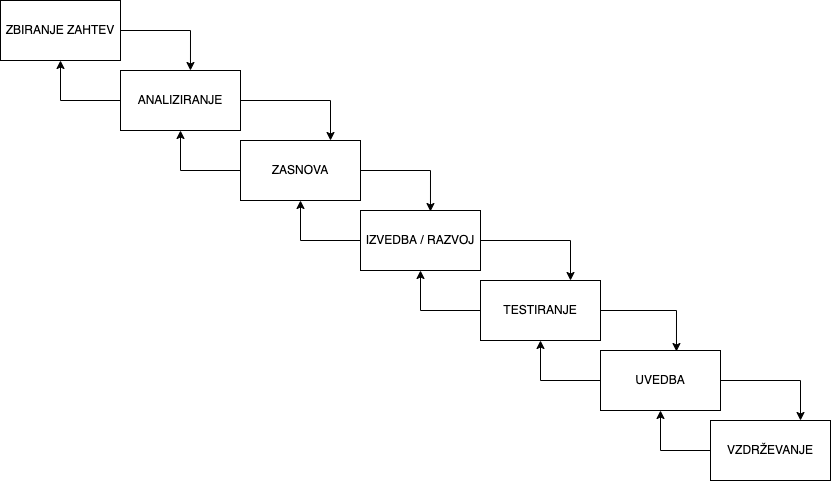
\includegraphics[width=1\textwidth]{slike/waterfall.png}
\end{center}
\caption{ Vizualizacija sedmih faz, prikazanih z grafom }
\label{waterfall-phases}
\end{figure}
\section{Nadzor različic}

Orodje, ki upravlja in sledi različnim verzijam programske kode ali drugih podatkov, ki so lahko predstavljeni v bitih, je znano kot sistem za verzioniranje podatkov. V angleščini poznamo vec izrazov, ki se navezujejo na omenjeno orodje, to so version control system (VCS), source code manager (SCM), revision control system (RCS) in se nekaj drugih permutacij besed “revision,” “version,” “code,” “content,” “control,” “management,” in “system.”.

Najlažje si je to predstavljati kot, nekakšno podatkovno bazo, ki hrani vse verzije nekih podatkov in nam prikazuje razliko med verzijami. Ponavadi so ti podatki shranjeni nekje na strežniku, da lahko do njih dostopajo vsi, ki delajo z njimi. Torej če delamo spletno stran, lahko tako vidimo kako se spletna stran razvija. Naprimer neka stran ima v verziji v0.1 slepo besedilo (Lorem ipsum), če to primerjamo z verzijo v1.0, kjer je že prava vsebina opazimo spremembo besedila. Shranijo se tudi krajša sporočila, ki omogočajo lažji pregled nad zgodovino sprememb in natančen vpogled kdo je naredil spremembo in kdaj je bila sprememba narejena.

\begin{figure}[h]
\begin{center}
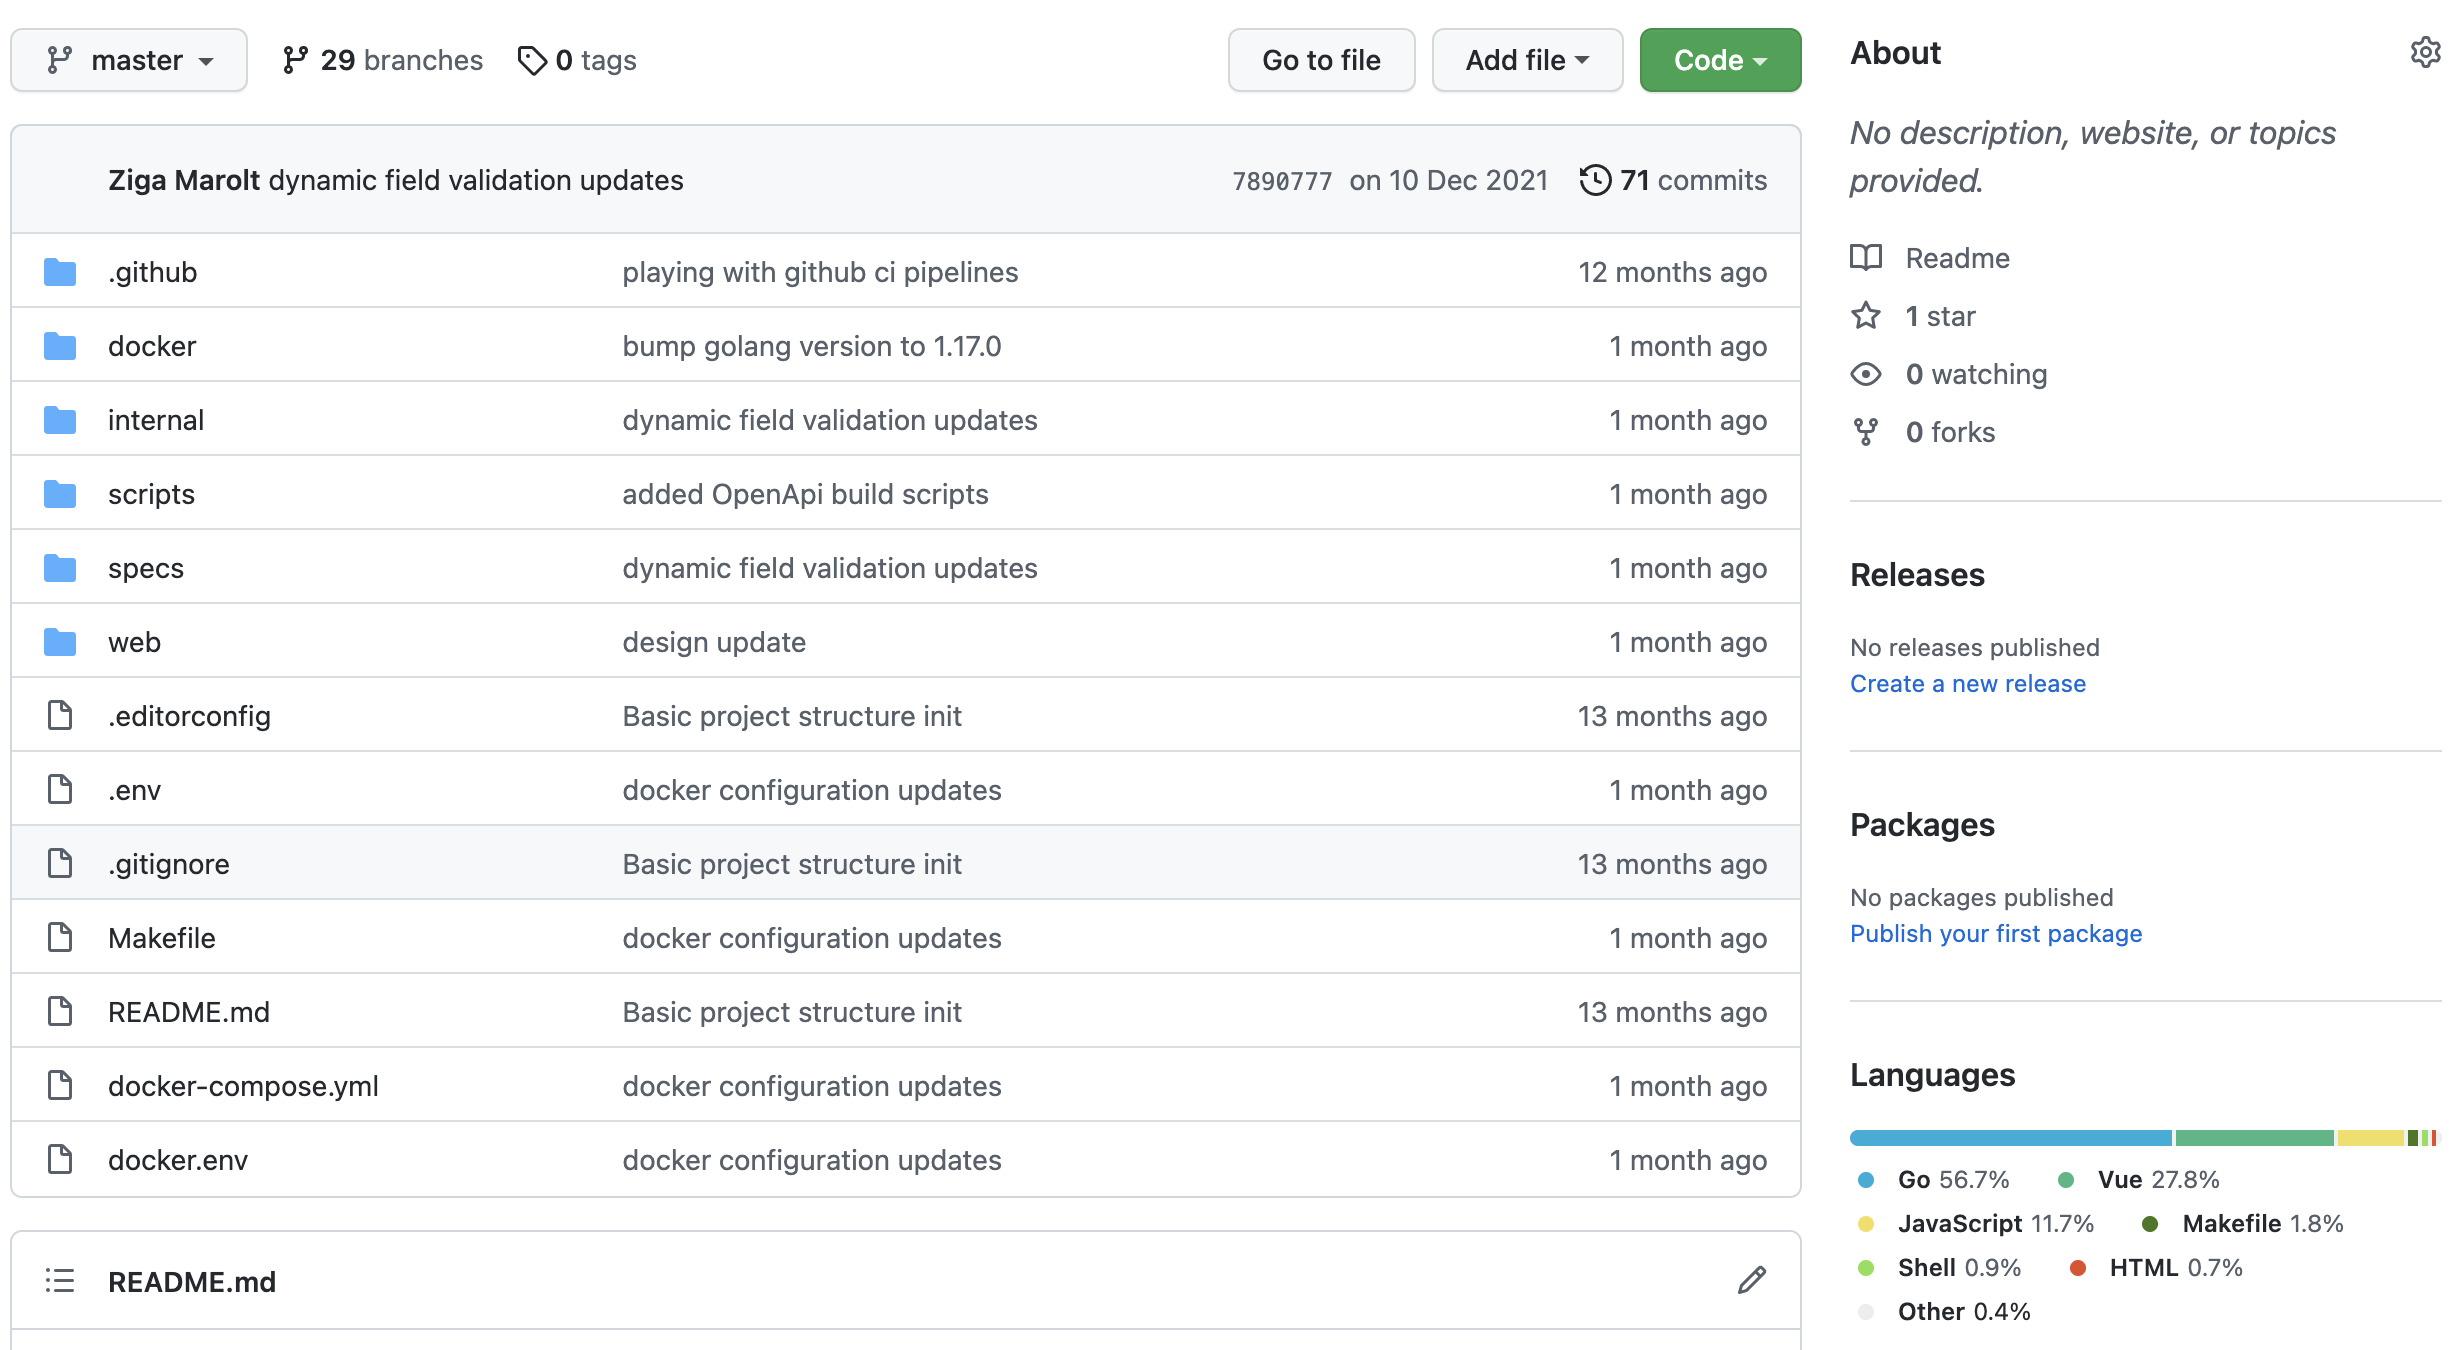
\includegraphics[width=1\textwidth]{slike/github.png}
\end{center}
\caption{ Prikaz Github repozitorija }
\label{github}
\end{figure}

\section{Zemljevid strani}
Aplikacija je sestavljena iz strani, katere lahko uporabnik dostopa iz različnih delov aplikacije. Stran ki jo uporabniki obiščejo najprej je pozdravna stran, ki je namenjena predstavitvi same aplikacije. Preko te strani uporabnik dostopa do ostalih delov aplikacije, katere bomo opisali v nadaljevanju.

\begin{description}
\item Definicije strani: \
	\begin{itemize}
        \item \textbf{Registracija}: ustvarjanje novega uporabnika
		\item \textbf{Prijava}: obrazec za overjanje uporabnika
		\item \textbf{Pozabljeno geslo}: nastavitev novega gesla uporabniku
		\item \textbf{Uporabniki}: seznam vseh uporabnikov v sistemu
		\begin{itemize}
		    \item urejanje: obrazec za urejanje uporabnika
		    \item brisanje: deaktiviranje uporabnika
		\end{itemize}
		\item \textbf{Publikacije}: seznam vnesenih publikacij
		\begin{itemize}
		    \item urejanje: obrazec za urejanje obstoječe publikacije
		    \item brisanje: odstranitev publikacije iz sistema
		    \item dodajanje: obrazec za kreiranje nove publikacije v sistem
		    \item iskanje: iskanje po naslovu 
		    \item prenos datoteke: prenos pripete datoteke k publikaciji
		\end{itemize}
		\item \textbf{Metode}: seznam vseh vnesenih metod v sistemu
		\begin{itemize}
		    \item urejanje: obrazec za urejanje obstoječe metode
		    \item brisanje: odstranitev metode iz sistema
		    \item dodajanje: obrazec za kreiranje nove metode
		\end{itemize}
		
		\item \textbf{Viri}: seznam vseh dodanih virov v sistem
		\begin{itemize}
		    \item urejanje: obrazec za urejanje obstoječega vira
		    \item brisanje: odstranitev vira iz sistema
		    \item dodajanje: obrazec za kreiranje novega vira
		\end{itemize}
		
		\item \textbf{Živila}: seznam vseh dodanih živil v sistemu
		\begin{itemize}
		    \item urejanje: obrazec za urejanje obstoječega živila
		    \item brisanje: odstranitev živila iz sistema
		    \item dodajanje: obrazec za kreiranje novega živila
		\end{itemize}
		
		\item \textbf{Avtorji}: seznam vseh dodanih avtorjev v sistemu
		\begin{itemize}
		    \item urejanje: obrazec za urejanje obstoječega avtorja
		    \item brisanje: odstranitev avtorja iz sistema
		    \item dodajanje: obrazec za kreiranje novega avtorja
		\end{itemize}
		
		\item \textbf{Dinamični podatki}: seznam vseh definiranih dinamičnih podatkov v sistemu
		\begin{itemize}
		    \item urejanje: obrazec za urejanje obstoječega podatka
		    \item brisanje: odstranitev podatka iz sistema
		    \item dodajanje: obrazec za kreiranje novega podatka
		\end{itemize}
		
		\item \textbf{Iskalnik}: stran za iskanje z različnimi parametri nad vnešenimi publikacijami
	\end{itemize}
\end{description}

\begin{figure}[h]
\begin{center}
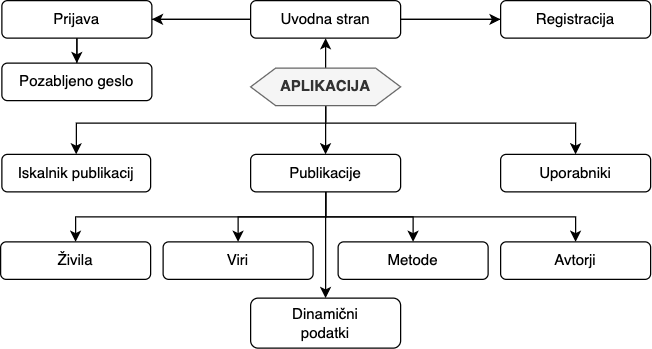
\includegraphics[width=1\textwidth]{slike/page-map.png}
\end{center}
\caption{ Zemljevid strani }
\label{sitemap}
\end{figure}

Za lažjo predstavitev medsebojnih povezav, so na sliki \ref{sitemap} prikazane povezave med posameznimi stranmi aplikacije med katerimi uporabnik lahko navigira.


\section{Infrastruktura}
Uporaba programske opreme je zapletena. Pred namestitvijo je potrebno razmisliti, kateri operacijski sistem se bo uporabljal, katera so orodja, ki jih programska oprema potrebuje in še vrsto drugih vprašanj. Večina računalnikov ima že nameščenih in zagnanih več aplikacij. In večina aplikacij je odvisna od druge programske opreme. Kaj se zgodi, če dve ali več aplikacij, ki so nameščene na računalniku, ne delujejo dobro skupaj? Pride do problema, ki pa ga ni tako enostavno odpraviti. Stvari postanejo bolj zapletene, če si aplikacije med sabo delijo skupne vire. 

Na našem projektu smo se hoteli izogniti nevšečnostim z oteženim postavljanjem projekta, zato smo se odločili oporabili orodje za izoliranje okolja. Virtualizacija je postopek, ki strojni ali programski vir preslika v navidezni vir, tega pa potem odjemalec koristi kot pravi vir. Pomembna prednost uporabe virtualizacije je prenostljivost. Z njo lahko dosežemo enake pogoje za izvajanje programske opreme na različnih strojnih opremah, in ravno to si želimo doseči.

V našem projektu smo se odločili uporabili orodje Docker. Orodje nam zagotavlja tako imenovano abstrakcijo, da poenostavljeno delamo z zapletenimi stvarmi in nudi enako okolje vsem uporabnikom, ki delujejo na istem projektu, ne glede na uporabljen operacijski sistem. 

\begin{figure}[h]
\begin{center}
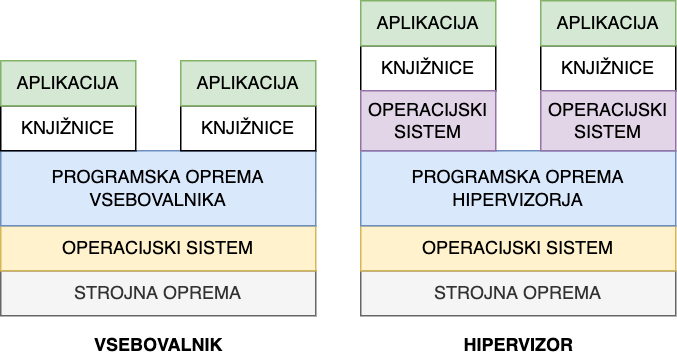
\includegraphics[width=0.75\textwidth]{slike/docker-vs-vm.png}
\end{center}
\caption{ Prikaz razlike med virtualnim strojem in Docker vsebovalnik }
\label{docker-vs-vm}
\end{figure}

\subsection{Docker}
Docker je trenutno najbolj priljubljena rešitev vsebnika. Ponuja številne funkcije in je podprt iz strani ostalih sistemov, kot so naprimer orodja za orkestracijo. V osnovi gre za izolacijo procesov in virtualizacijo virov, do katerih procesi dostopajo. Omogoča izoliranje aplikacije od infrastrukture, za hitro dostavljanje programske opreme. \cite{linuxcontainers} 

Docker je odvisen od jedra Linuxa, kar pomeni, da ne deluje v sistemu Windows ali macOS. V tem primeru je potreben zagon v virtualnem stroju, ki vsebuje jedro $Linuxa$. \cite{docker-in-action}

Konfiguriranje slike vsebnika zahteva ustvarjanje konfiguracijske datoteke, ki je ponavadi znotraj projekta in se imenuje $Dockerfile$. To je tekstovna datoteka, ki opisuje zahteve posameznega programa, kot so osnovna slika za izvajanje (npr. slika ki omogoča izvajanje Go programov), ukazi za zagon (npr. namestitev), vrata, na katerih bo aplikacija poslušala, in tako naprej.

\begin{figure}[h]
\begin{center}
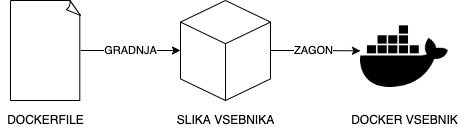
\includegraphics[width=0.75\textwidth]{slike/docker-flow.png}
\end{center}
\caption{ Prikaz gradnje docker vsebovalnikov }
\label{password-reset-form}
\end{figure}

Dockerjeve slike imajo nekakšen sistem odvisnosti. Slika lahko razširi drugo sliko, ki sama lahko razširi še eno. Ko izvaja namestitev, bo Docker prenesel vsako plast in jo predpomnil, tako da bodo naslednje namestitve hitrejše. Da se datotečni sistemi vsake plasti združijo eno na drugo poskrbi sistem UnionFS.  Slike so enote, ki jih je mogoče pošiljati v ekosistemu Docker. Docker ponuja nabor infrastrukturnih komponent, ki poenostavljajo distribucijo slik vmestnikov. Te komponente so registri in indeksi. Na voljo za uporabo je javno dostopno infrastruktura, ki jo nudi $Docker Inc.$, uporabi pa se lahko tudi privatni register, ki ga gostimo sami (naprimer $GitLab$ register).

Vsebniki so skupina procesov v operacijskem sistemu z jedrom Linux, katerim upravlja računske vire z nadzornimi skupinami in zagotavlja izolacijo virov z uporabo imenskih prostorov. Ob zagonu vsebnika se uporabni vsebniška slika (angl. container image) v kateri so zapisane informacije o izvajanju programske opreme in preko katere Docker tudi priklopi nov, prazen bralno-pisalni datotečni sloj. Slika se ustvari s postopkom gradnje, ki je zapisan v datoteki $Dockerfile$. 

V kodi spodaj (\ref{lst:dcb-snipet}), je prikazan primer grajenja slike, ki smo jo uporabili pri razvoju zalednega dela naše aplikacije.
\begin{lstlisting}[language=bash, style=mystyle,caption={Grajenje slike docker vmestnika},label=lst:dcb-snipet]
$ docker build .          
[+] Building 69.1s (9/9)                             FINISHED
 => [internal] load build definition from Dockerfile    0.1s
 => => transferring dockerfile: 180B                    0.0s
 => [internal] load .dockerignore                       0.0s
 => => transferring context: 2B                         0.0s
 => [internal] load metadata for golang:1.17            2.7s
 => [1/2] FROM golang:1.17@sha256:39953c7c7             60.0s
 => => resolve golang:1.17@sha256:39953c7c7             0.0s
 => => sha256:0e29546d54 54.92MB / 54.92MB              27.2s
 => => extracting sha256:0e29546d541                    4.5s
 => => sha256:6432567af305a4304605a3 154B / 154B        34.4s
 => [internal] load build context                       0.0s
 => => transferring context: 121B                       0.0s
 => [2/2] COPY start.sh /                               0.0s 
 => exporting to image                                  0.2s 
 => => exporting layers                                 0.2s 
 => => writing image sha256:96d781a9030                 0.0s 
\end{lstlisting}
\section{Arthitektura}
Arhitekturna zasnova močno vpiva na delovanje in razvoj aplikacije. Vsak arhitekturni koncept ima svoje prednosti in slabosti. Na projektu smo hoteli spoznati arhitekturo mikrostoritev. Ta vrsta arhitekture definira aplikacijo, sestavljeno iz majhnih samostojnih enot. Vsaka enota ima točno določeno funkcijo in lahko deluje neodvisno od ostalih enot.

Arhitekturni koncept mikrostoritev je pristop k razvoju ene same aplikacije kot zbirke majhnih storitev, od katerih vsaka deluje v svojem procesu in komunicira z enostavnimi mehanizmi, kot je naprimer HTTP API. Te storitve so zgrajene na podlagi poslovnih zmogljivosti in jih je mogoče neodvisno uvesti s popolnoma avtomatiziranimi stroji za uvajanje. Obstaja minimalno centralizirano upravljanje teh storitev, ki so lahko napisane v različnih programskih jezikih in uporabljajo različne tehnologije za shranjevanje podatkov. \cite{mfowler-microservices}

Kot je razvidno na sliki \ref{app-architecture}, smo v naši aplikaciji definirali dve storitvi. Vsaka storitev ima svoja opravila in je neodvosna od ostalih enot. Za medsebojno komunikacijo se uporablja protokol HTTP.

\begin{figure}[h]
\begin{center}
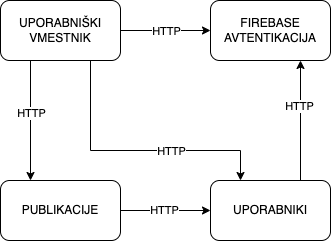
\includegraphics[width=0.5\textwidth]{slike/architecture.png}
\end{center}
\caption{ Arhitektura mikrostoritev naše aplikacije }
\label{app-architecture}
\end{figure}

Arhitektura kode sledi uporabi dobre prakse, z uporabo vzorcev, ki nam pomagajo pri strukturiranju same kode. Uporabljamo vzorec repozitorija, ki nam pomaga ločiti logiko za pridobivanje podatkov. S tem enostavno ločimo domensko logiko, od logike za poizvedbo podatkov. Za vsako zbirko podatkov smo definirali vmestnik. Vmestnik definira metode, ki so lahko implementirane na različne načine. Ta način nam omogoča enostavno spreminjanje implementacije, v primeru, da hočemo zamenjati podatkovno bazo. 

Za potrebe aplikacije smo vmestnike implementirali z implementacijo PostgreSQL podatkovne baze. 
\begin{lstlisting}[language=go, style=mystyle,caption={Vmestnik, ki definira repozitorij za publikacije},label=lst:article-repository]
// ArticleRepository defines the datastore handling persisting Article records.
type ArticleRepository interface {
	Create(ctx context.Context, article *Article, callback ArticleCallbackFn) (*Article, error)
	Delete(ctx context.Context, id utils.BINARY16) error
	Find(ctx context.Context, id utils.BINARY16) (*Article, error)
	Update(ctx context.Context, article *Article, callback ArticleCallbackFn) (*Article, error)

	// Paginate ...
	Paginate(ctx context.Context, opts PageOpts, filters ArticleFilterOpts) ([]Article, error)

	AssignAuthors(ctx context.Context, article *Article, authors []*Author, callback ArticleCallbackFn) error
	AssignFoodstuffs(ctx context.Context, article *Article, foodstuffs []*Foodstuff, callback ArticleCallbackFn) error
	AssignMethods(ctx context.Context, article *Article, methods []*Method, callback ArticleCallbackFn) error
	AssignFile(ctx context.Context, uuid utils.BINARY16, fileUUID utils.BINARY16) error

	AddField(ctx context.Context, article *Article, field ArticleField) error
	GetExtras(ctx context.Context, uuid utils.BINARY16) ([]ArticleField, error)
}

// ArticleSearchRepository defines the datastore handling searching Article records.
type ArticleSearchRepository interface {
	Search(ctx context.Context, args SearchParams) (SearchResults, error)
}
\end{lstlisting}

\section{Programski jezik Go}

\verb=Go= (ali golang) je odprtokodni programski jezik, razvit iz strani ameriške kooproracije Google. Pobudniki razvojo so bili Robert Griesemer, Ken Thomson, in Rob Pike. Sprva je bil uporabljen le za interno uporabo, leta 2009 pa so ga ponudili kot odprto kodni programski jezik širši publiki. 
 
Kljub temu, da je programski jezik Go, jezik za splošno uporabo, je njegova primarna uporabna namenjena pisanju sistemskih orodij, spletnih storitev in programov, ki veliko komunicirajo preko  spletnega omrežja. Primeren je tudi za učenje prvega programskega jezika, zaradi njegove enostavnosti in pristopov. Definiranih, oziroma rezerviranih je le 25 ključnih besed, kar pomeni, da si je veliko lažje zapomniti jezik, in se je potrebno naučiti le konceptov.

Čeprav Go ni objektno usmerjen programski jezik, so njegovi vmesniki zelo vsestranski in omogočajo posnemanje nekaterih zmožnosti objektno usmerjenih jezikov, kot so polimorfizem, enkapsulacija in sestava.

Go ima tudi zmožnosti sočasnosti z uporabo preprostega modela sočasnosti, ki se izvaja z uporabo go-rutin in kanalov. Go upravlja niti operacijskega sistema namesto nas in ima zmogljiv izvajalni čas. To omogoča ustvarjanje lahkih delovnih enot (goroutine), ki med seboj komunicirajo s pomočjo kanalov.
 

 
% \section{Metrike}

% V IT in računalništvu v oblaku je opaznost zmožnost merjenja trenutnega stanja sistema na podlagi podatkov, ki jih ustvari, kot so dnevniki, meritve in sledi.

% Opazovanost je odvisna od telemetrije, ki izhaja iz instrumentov, ki prihajajo iz končnih točk in storitev v vaših računalniških okoljih v več oblakih. V teh sodobnih okoljih vsaka komponenta strojne opreme, programske opreme in infrastrukture v oblaku ter vsak vsebnik, odprtokodno orodje in mikrostoritev ustvari zapise o vsaki dejavnosti. Cilj opazljivosti je razumeti, kaj se dogaja v vseh teh okoljih in med tehnologijami, tako da lahko odkrijete in razrešite težave, da bodo vaši sistemi učinkoviti in zanesljivi, vaše stranke pa zadovoljne.

% Organizacije običajno izvajajo opazljivost s kombinacijo instrumentacijskih metod, vključno z odprtokodnimi instrumentacijskimi orodji, kot je OpenTelemetry.

% Številne organizacije sprejmejo tudi rešitev opazovanja, ki jim pomaga odkriti in analizirati pomen dogodkov za njihovo delovanje, življenjske cikle razvoja programske opreme, varnost aplikacij in izkušnje končnih uporabnikov.

% Opaznost je v zadnjih letih postala bolj kritična, saj so okolja, ki izvirajo iz oblaka, postala bolj zapletena in je vedno težje določiti možne temeljne vzroke za okvaro ali nepravilnost. Ko ekipe začnejo zbirati in delati z opazovanimi podatki, spoznavajo tudi njegove koristi tudi za poslovanje.

% Ker se storitve v oblaku zanašajo na edinstveno porazdeljeno in dinamično arhitekturo, se lahko opaznost včasih nanaša tudi na posebna programska orodja in prakse, ki jih podjetja uporabljajo za razlago podatkov o zmogljivosti v oblaku. Čeprav nekateri ljudje mislijo, da je opaznost modna beseda za prefinjeno spremljanje zmogljivosti aplikacij (APM), je pri primerjavi opaznosti in spremljanja treba upoštevati nekaj ključnih razlik. \cite{ot-what-is-observability}
\section{Spletni strežnik}

Spletni strežnik (angl. Web Server) je računalniški sistem, ki obdeluje zahteve preko protokola \verb=HTTP=. Izraz spletni strežnik se lahko nanaša na celoten sistem ali posebej na programsko opremo, ki sprejema in nadzira zahteve HTTP. Primarna funkcija spletnega strežnika je shranjevanje, obdelava in pošiljanje spletnih strani odjemalcem. Predložene strani so najpogosteje dokumenti HTML, ki poleg besedilne vsebine vključujejo tudi slike, CSS prdloge in skripte. 

Glavna naloga spletnega strežnika je prikazovanje vsebine spletne strani. Če spletni strežnik ni izpostavljen javnosti in se uporablja interno, se imenuje \sn{intranetni strežnik}. Strojna oprema spletnega strežnika je povezana z internetom in omogoča izmenjavo podatkov z drugimi povezanimi napravami, medtem ko programska oprema spletnega strežnika nadzoruje, kako uporabnik dostopa do gostiteljskih datotek.

% Primer spletnega strežnika v programskem jeziku Go (\ref{lst:ws-go}), dosegljivega na naslovu  \url{http://localhost:8080/}.
\begin{lstlisting}[language=go, style=mystyle,caption={Spletni strežnik v programskem jeziku Go},label=lst:ws-go]
package main

import (
    "fmt"
    "log"
    "net/http"
)

func handler(w http.ResponseWriter, r *http.Request) {
    fmt.Fprintf(w, "Pozdravljen svet!")
}

func main() {
    http.HandleFunc("/", handler)
    log.Fatal
}
\end{lstlisting}


Do programske opreme spletnega strežnika se dostopa preko domenskih imen spletnih mest in zagotavlja dostavo vsebine spletnega mesta uporabniku, ki je poslal zahtevek. Strežnik HTTP lahko razume HTTP in URL-je. Kot strojna oprema je spletni strežnik računalnik, ki shranjuje programsko opremo spletnega strežnika in druge datoteke, povezane s spletnim mestom, kot so dokumenti HTML, slike in datoteke JavaScript.

Dinamični spletni brskalniki poleg spletnega strežnika vključujejo tudi druge programske opreme, kot naprimer aplikacijski strežnik in podatkovno bazo podatkov. Šteje se za dinamično, ker je aplikacijski strežnik mogoče uporabiti za konstruiranje odgovorov na zahtevek, preden se pošljejo v brskalnik. Spletni strežnik lahko generira vsebino, ko je zahtevana iz baze podatkov. Čeprav je ta postopek bolj prilagodljiv, je tudi bolj zapleten.

%%%%%%%%%%%% Komunikacija med storitvami %%%%%%%%%%%% 
\section{Komunikacija in dokumentacija}
Za komunikacijo z zalednim delom aplikacije uporabljamo \verb=HTTP= (Hypertext Transfer Protocol) protokol. \verb=HTTP= je brezstanjski protokol aplikacijskega sloja, ki skrbi za komunikacijo med odjemalcem in strežnikom. Deluje po protokolu \verb=zahtevek-odgovor= (angl. request–response ali request–reply) v modelu odjemalec-strežmik (\ref{communication-flow}). Zahtevki se izvajajo sinhrono, kar pomeni, da je povezava med odjemalcem in strežnikom odprta toliko časa, dokljer strežnik ne odgovori z podatki, oziroma do neke časovne omejitve. \cite{http-rfc}


\begin{figure}[h]
\begin{center}
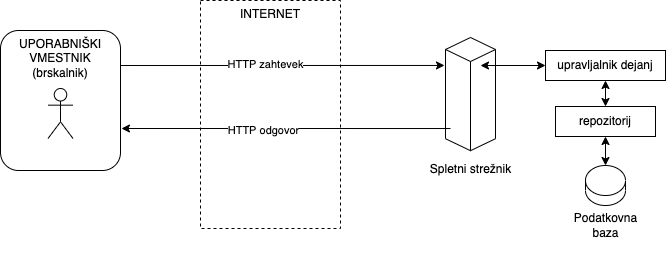
\includegraphics[width=0.75\textwidth]{slike/communication.png}
\end{center}
\caption{ Prikaz komunikacije po protokolu zahtevek-odgovor }
\label{communication-flow}
\end{figure}

Za komunikacijo z zalednim delom aplikacije smo definirali aplikacijski programski vmestnik (API), z uporabo protokola HTTP. Vmestnik je arhitekturno predstavljen kot REST API, kar pomeni, da je vsak vir predstavljen kot spletna storitev z enooznačnim naslovem URL. Za pridobivanje in urejanje podatkov uporabljamo standardne HTTP metode: GET, POST, PUT, DELETE. Sistemi, ki uporabljajo REST pristop stremijo k hitri, odzivni in stabilni komunikaciji med odjemalcem in strežnikom.


\begin{description}
    \item Primer definiranih virov za pridobivanje, urejanje, brisanje in kreiranje publikacij v sistemu:
    \begin{itemize}
        \item \textbf{GET /articles/list} - Vrni listo publicitacij
        \item \textbf{POST /articles/add} - Shrani novo publicitacijo
        \item \textbf{GET /articles/:uuid/get} - Vrni publicitacijo za dodeljen ID 
        \item \textbf{DELETE /articles/:uuid/delete} - Izbriši publicitacijo za dodeljen ID
        \item \textbf{PUT /articles/:uuid/update} - Osveži obstoječo publicitacijo
        \item \textbf{POST /articles/:uuid/upload-files} - Pripni datoteko k publicitaciji
        \item \textbf{DELETE /articles/:uuid/files/:file-uuid} - Odstrani datoteko od publicitacije
    \end{itemize}
\end{description}

Pri definiranju komunikacijskega vmestnika smo sledili znanemu standardu \verb=OpenApi 3.0=. Kreirali smo specifikacijske datoteke, kjer je definiran vsak klic, ki ga je mogoče izvesti na zaledni del. Te specifikacije nam pomagajo pri grajenju dokumentacije, v našem primeru pa tudi grajenje kode, ki poskrbi za komunikacijo (\ref{swagger-docs}).

\begin{figure}[h]
\begin{center}
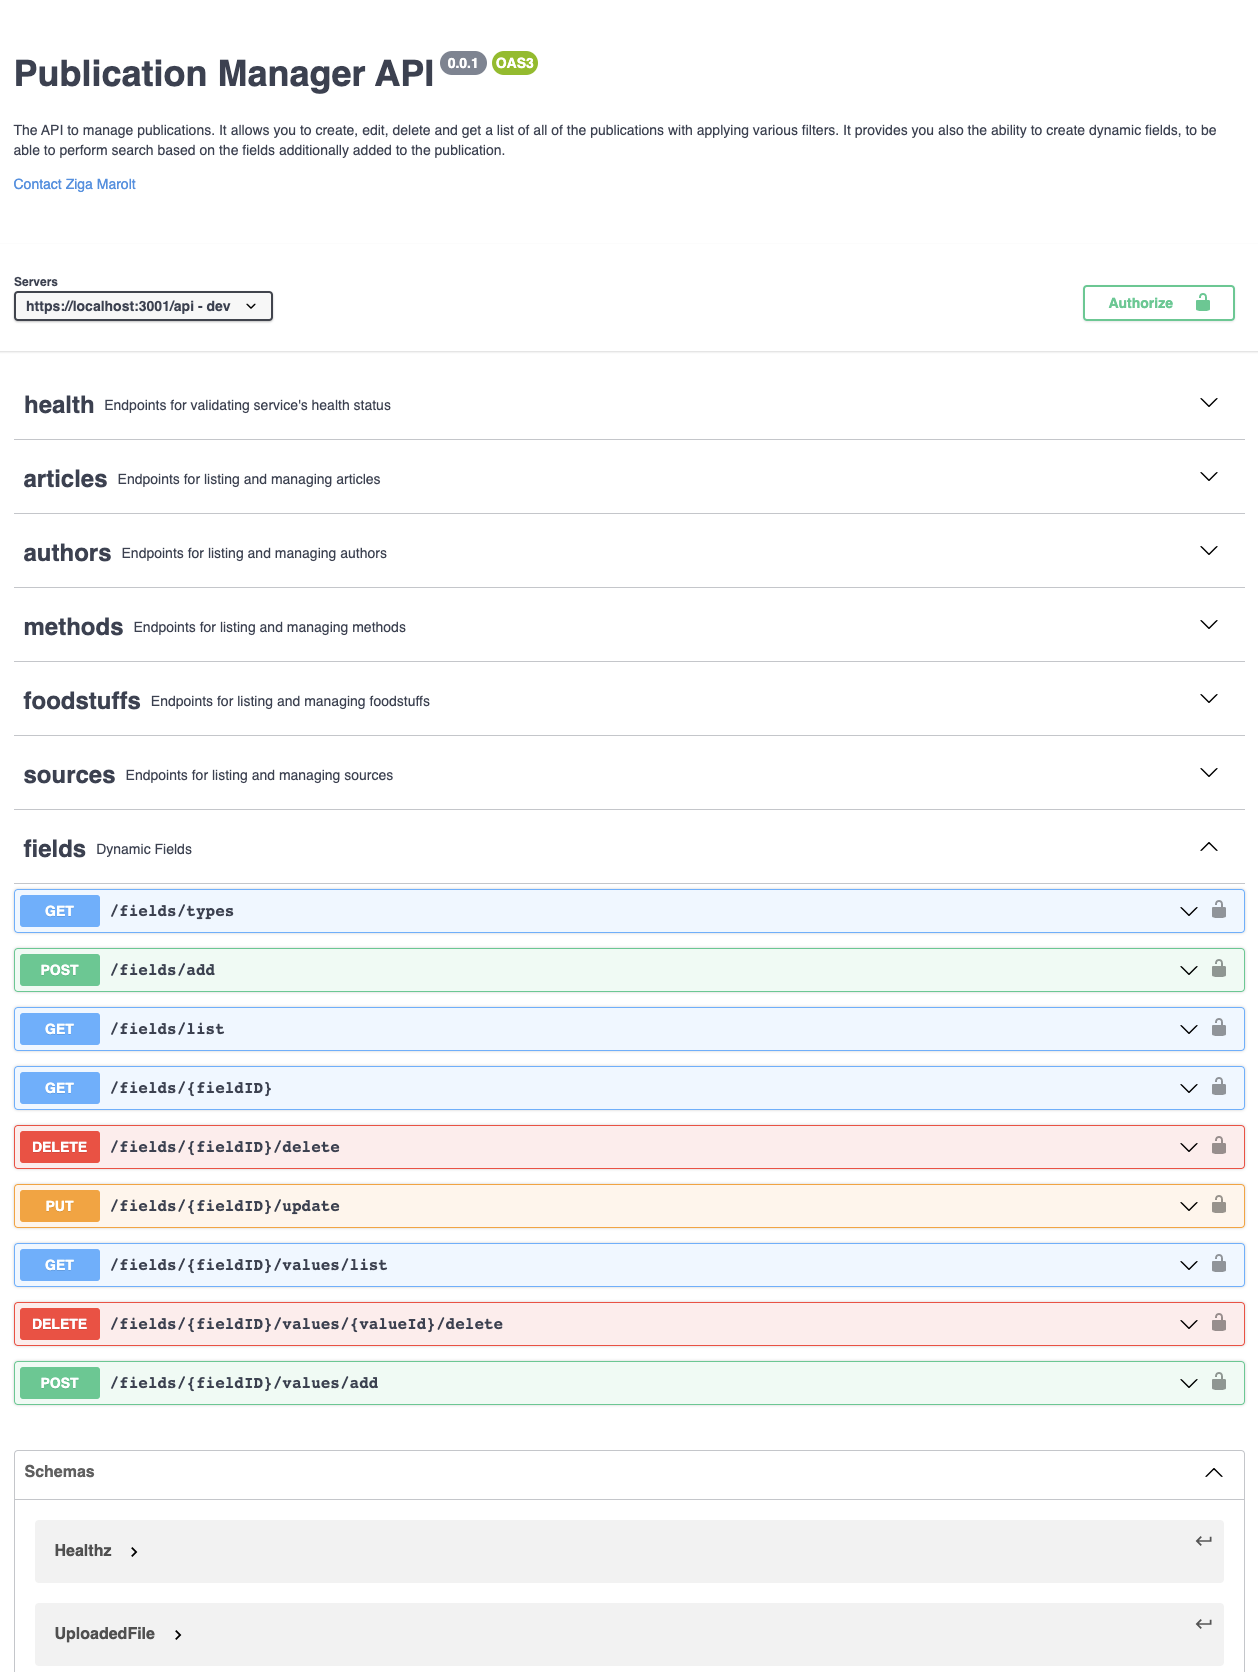
\includegraphics[width=1\textwidth]{slike/documentation.png}
\end{center}
\caption{ Dokumentacija z orodjem Swagger }
\label{swagger-docs}
\end{figure}

Glede na specifikacije vmestnika, zgeneriramo kodo, ki poskrbi za komunikacijo med sistemi. Generirana koda je enostavna za uporabo in je postala dobra praksa saj s tem tudi zagotovimo, da je dokumentacija komunikacijskega vmestnika ves čas pravilna. 

Za zaledni del uporabimo generator \verb=Swagger= \cite{swagger-codegen}, s katerim pridobimo osnovno kodo za HTTP strežnik, ki streže podatke odjemalcem. Omogoča nam osnovno validacijo podatkov, ki so poslani v zahtevku in le te pretvori v primerno strukturo, s katero je enostavno manipulirati dalje v aplikaciji. 

Za čelni del zgeneriramo javascript odjemalce z \verb=OpenApi= generatorjem, ki poskrbijo za komunikacijo z strežnikom, na zalednem delu. S tem nam ni potrebno skrbeti, da bi skonstruirali zahtevek v napačni obliki.

Da je delo enostavno, smo naredili skripte, ki poskrbi da se zgenerira željena koda, za čelni in zaledni del aplikacije (\ref{lst:generator-script}).

\begin{lstlisting}[language=bash, style=mystyle,caption={Skripta, ki poskrbi za generiranje kode za posamezno storitev},label=lst:generator-script]
#!/bin/bash
set -e

readonly service="$1"

readonly docker_image="openapitools/openapi-generator-cli:v5.3.0"

docker run --rm --env "JAVA_OPTS=-Dlog.level=error" -v "${PWD}:/local" \
  "$docker_image" generate \
  -i "/local/api/openapi/$service.yml" \
  -g javascript \
  -o "/local/web/src/services/clients/$service"
\end{lstlisting}

Za izmenjavo podatkov med odjemalcem in strežnikom uporabljamo JSON strukturo. JSON (angl. JavaScript Object Notation) je preprosta oblika za izmenjavo podatkov, ki je neodvisna od programskega jezika. Zaradi besedne zasnove je enostaven za branje in pisanje tako ljudem kot tudi računalnikom \cite{json-rfc}.

\begin{lstlisting}[language=bash, style=mystyle,caption={Primer izvedbe API klica in odgovora},label=lst:api-call-example]
 curl --request POST \
 --url https://localhost:3001/api/authors/{authorID}/update \
 --header 'Authorization: Bearer ==token==' \
 --header 'Content-Type: application/json' \
 --data '{
    "name": "John Doe"
 }'
\end{lstlisting}

Komunikacija pa je lahko uspešna ali ne, zato je potrebno odjemalcu odgovoriti z ustrezno kodo, kot je definirano v standardu HTTP. Statuse lahko razdelimo v razlčne grupe, ki predstavljajo napake storjene na strani odjemalca (4xx), napake storjene na strani strežnika (5xx) in uspešno obdelane zahtevke (2xx). V tabeli ~\ref{table:http-codes} so prikazane vse napake, ki jih aplikacija lahko vrne. 
\begin{table}[h]
\begin{tabular}{ll}
\textbf{Koda napake} & \textbf{Pomen}                                                    \\
200                  & $OK$ - Zahtevek je uspešno izveden                                  \\
400                  & $Bad Request$ - Zahtevek ni veljaven                                \\
401                  & $Unauthorized$ - Žeton ni veljaven                                  \\
403                  & $Forbidden$ - Ni zadostnih pravic                                   \\
404                  & $Not Found$ - Vir ne obstaja                                        \\
422                  & \begin{tabular}[c]{@{}l@{}}$Unprocessable Entity$ - Zahtevek vsebuje neveljavne \\ podatke \end{tabular}   \\
429                  & \begin{tabular}[c]{@{}l@{}}$Too Many Requests$ - Narejenih preveč zahtevkov v \\ časovnem obdobju\end{tabular} \\
500, 502, 503, 504   & $Internal Server Error$ - Napaka na zalednem sistemu
\end{tabular}
\caption{Seznam napak, ki jih vrača strežnik}
\label{table:http-codes}
\end{table}

\section{Avtentikacija in avtorizacija}

Skoraj vsaka aplikacija zahteva določeno raven sistema avtorizacije. V nekaterih primerih je dovolj, da potrdimo nabor uporabniškega imena/gesla z našo tabelo Users, vendar pogosto potrebujemo bolj natančen model dovoljenj, da nekaterim uporabnikom omogočimo dostop do določenih virov in jih omejimo pred ostalimi. 

V aplikaciji imamo definirane tri različne nivoje uporabnikov. Implementacija je narejena na poznanem konceptu nadzora dostopa na podlagi vlog (angl. Role-based access control - RBAC).

Za preverjanje pristnosti uporabnika med posameznimi zahtevki, uporabljamo žeton JWT (JSON Web Token), v kateremu je zapisan identifikator uporabnika in njegova vloga. Žeton je brezstanjski, kar pomeni, da ni nikjer shranjen. To nam omogoča izdelavo ločenih sistemov, ki niso vezani na določeno shemo preverjanja pristnosti. Žeton je lahko ustvarjen kjer koli in porabljen v katerem koli sistemu, ki za podpis žetona uporablja isti skrivni ključ. Tako nam podatkov o uporabniku ni potrebno vedno znova, ob vsakem zahtevku preveriti s podatki v bazi.

Vsak zahtevek poslan preko aplikacijskega programskega vmestnika mora v glavi vsebovati žeton, predstavljen kot \verb=Bearer= žeton. V čelnem sistemu, smo naredili različne kliente, ki komunicirajo z zalednim sistemom. Ti klienti skrbijo, da se žeton pošlje v glavi vsakega zahtevka. Ker ima žeton določeno življensko dobo, je bilo potrebno poskrbeti tudi za osveževanje tega žetona (glej sliko \ref{token-flow}). Ob vsaki spremembi žetona se klientom nastavi novo vrednost žetona, s tem poskrbimo, da je žeton ves čas delujoč in veljaven (glej kodo \ref{lst:auth-set-token}).

\begin{figure}[h]
\begin{center}
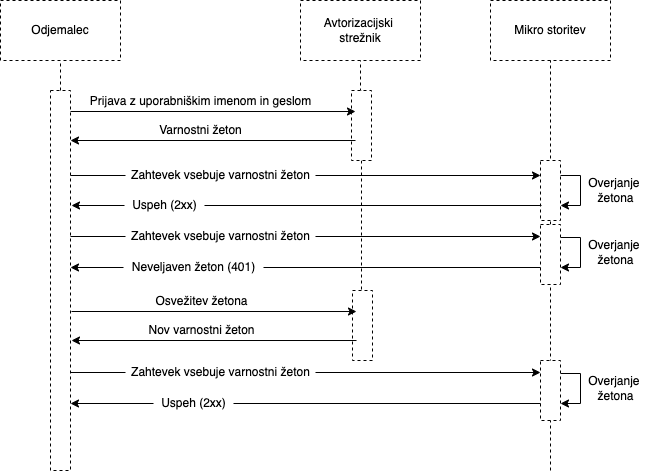
\includegraphics[width=0.75\textwidth]{slike/token-flow.png}
\end{center}
\caption{ Diagram prikazuje komunikacijo z uporabo žetona (JWT) }
\label{token-flow}
\end{figure}


\begin{lstlisting}[style=mystyle,caption={Izsek kode za nastavljanje žetona posameznemu klentu},label=lst:auth-set-token]
export function setApiClientsAuth(idToken) {
    users.authentications.bearerAuth.accessToken = idToken;
    fields.authentications.bearerAuth.accessToken = idToken;
    ...
}
\end{lstlisting}


V zalednem sistemu se ob vsakem zahtevku, sproži akcija za overjanje, poznano kot \verb=middleware= (glej kodo \ref{lst:auth-middleware}), z uporabo skrivnega ključa, s katerim je bil žeton tudi zgeneriran, overimo žeton. V primeru da žeton ni veljaven odgovorimo z ustreznim odgovorom, v tem primeru \verb=401 - Unauthorized=. 

V primeru, da je žeton veljaven, preberemo vrednost žetona, ki v našem primeru vsebuje identifikator uporabnika, uporabniško ime, poštni predal in vlogo uporabnika. S prebranimi vrednostmi kreiramo objekt uporabnika in nadaljujemo s procesiranjem zahtevka.

\begin{lstlisting}[language=go,style=mystyle,caption={Izsek kode za preverjanje pristnosti uporabnika},label=lst:auth-middleware]
func UserMiddleware(ctx context.Context, authService Service) MiddlewareFunc {
	return func(authToken string) (*User, error) {
			if !strings.HasPrefix(authToken, "Bearer ") {
			return nil, apierrors.Forbidden()
		}

		authToken = strings.TrimSpace(strings.Replace(authToken, "Bearer", "", 1))
		if authToken == "" {
			return nil, apierrors.Unauthorized()
		}

		token, err := authService.VerifyToken(ctx, authToken)
		if err != nil {
			return nil, apierrors.Unauthorized()
		}
		
		return &User{
			UID:         UID(token.UID),
			Email:       token.Claims["email"].(string),
			Role:        token.Claims["role"].(string),
			DisplayName: token.Claims["name"].(string),
		}, nil
	}
}
\end{lstlisting}

Preverjanje pravic se preveri v kontrolerju, ki vsebuje logiko kaj se zgodi z zahtevkom (glej kodo \ref{lst:auth-check-role}). Najprej preverimo, če je zahtevek od uporabnika, ki ima zadostne pravice za izvajanje tega zahtevka. V primeru, da uporabnik nima zadostnih pravic, mu odgovorimo z odgovorm \verb=403 - Forbidden=. V primeru, da uporabnik ima pravice, se izvede zahtevana operacija, v določenem servisu (angl. service).

\begin{lstlisting}[language=go,style=mystyle,caption={Izsek kode za preverjanje pravic uporabnika},label=lst:auth-check-role]
// DeleteUserHandler handles the delete user request
func (h *HttpHandler) DeleteUserHandler() users.DeleteUserHandlerFunc {
	return func(params users.DeleteUserParams, user *auth.User) middleware.Responder {

		// check if user has rights to perform this action
		if user.Role != string(domain.AdminRole) {
			return users.NewDeleteUserHandlerForbidden()
		}

		uuid, err := utils.StringToBinary16(string(params.UserID))
		if err != nil {
			return h.returnError(err)
		}
		u, err := h.app.Commands.DeleteUser.Handle(params.HTTPRequest.Context(), command.DeleteParamsCmd{
			UserUUID: uuid,
		})

		if err != nil {
			return h.returnError(err)
		}

		return users.NewUpdateUserNoContent()
	}
}
\end{lstlisting}

Pregled dostopov do posameznih delov aplikacje je nazorno predstavljeno z diagramom \ref{user-rights}.
\begin{figure}[h]
\begin{center}
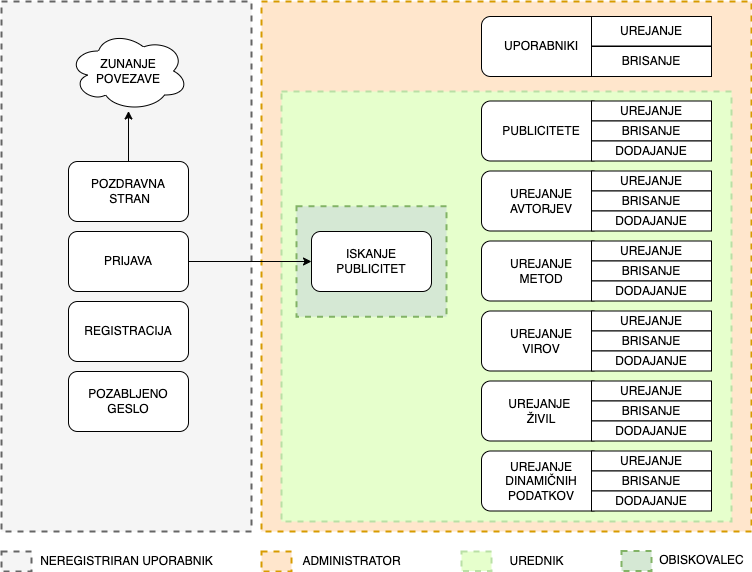
\includegraphics[width=0.75\textwidth]{slike/user_hierarchy.png}
\end{center}
\caption{ Pregled dostopa do posameznih strani in akcij glede na vlogo uporabnika }
\label{user-rights}
\end{figure}


\subsection{Firebase}
Firebase je zaledni del kot storitev (BaaS), ki jo nudi podjetje Google. Z orodji, ki jih Firebase ponuje, je programerjem olajšano delo pri razvoju in pa tudi pri vzdrževanju aplikacije. Orodja ki jih nudijo so avtentikacijsko orodje, orodje za testiranje, orodje za obveščanje strank in ostsala infrastrukturna orodja kot je podatkovna baza in  gostovanje. \cite{firebase-about}

Za potrebo naše aplikacije smo uporabili Firebase avtentikacijo. Avtentikacija temelji na žetonih, in zagotavlja izključene integracije z najpogostejšimi ponudniki, kot so Google, Facebook in Twitter, in ostali.

Omogoča nam uporabo zahtevkov po meri, ki jih bomo izkoristili za izgradnjo prilagodljivega API-ja, ki temelji na vlogah. V zahtevke lahko nastavimo katero koli vrednost JSON (npr. \{ "vloga": 'administrator' \} ali \{ "vloga": 'urednik' \}). Nastavljeni zahtevki so zapisani v žetonu, ki ga zgenerira Firebase.

Prihaja tudi z zelo velikodušno brezplačno kvoto, ki je za potrebo projekta vec kot dovolj. Storitev Firebase omogoča kreiranje neomejenega števila uporabnikov. Omejeno je število registriranih in izbrisanih uporabnikov v časovnem obdobju:

\begin{description}
\item Omejitve \cite{firebase-limits}:
	\begin{itemize}
		\item \textbf{Število registriranih uporabnikov} - neomejeno
		\item \textbf{Hitrost brisanja uporabnikov} - 10 uporabnikov/sekundo
		\item \textbf{Hitrost kreiranja uporabnikov} - 100 uporabnikov/IP/uro
	\end{itemize}
\end{description}


\section{Vue.js}
\label{vue-js-section}
Vue (prebran $/vju/$, kot angl. view) je odprtokodno, progresivno \verb=JavaScript= ogrodje (angl. framework), namenjeno izdelavi uporabniških vmesnikov in enostranskih aplikacij.

Vue.js ima postopoma prilagodljivo arhitekturo, ki se osredotoča na deklarativno upodabljanje in sestavo komponent. Jedrna knjižnica je osredotočena samo na vizualni sloj. Napredne funkcije, potrebne za zapletene aplikacije, kot so usmerjanje, upravljanje stanja in orodja za gradnjo, so na voljo prek uradno vzdrževanih podpornih knjižnic in paketov \cite{vue-js-what-is}.

\clearpage
\section{Shranjevanje podatkov}
Za potrebo po shranjevanju podatkov uporabljamo relacijsko podatkovno bazo \verb=PostgreSQL=. Relacijska podatkovna baza (RDBMS) uporablja podatkovno strukturo, ki nam omogoča identifikacijo in dostop do podatkov preko relacije med dvema entitetama. Podatke v relacijski podatkovni bazi, si lahko prdstavljamo kot tabele, z stolpci in vrsticami \cite{oracle-rdbms}.

Da so podatki shranjeni v popolni obliki, uporabljamo transakcije. Transakcija je atomična enota, s čimer zagotovimo da so vse poizvedbe izvedene uspešno. V primeru, da ena poizvedba ni bila uspešno izvedena, se vse poizvedbe storjene v isti transakciji povrnejo v stanje pred izvedbo. 

% Za enostaven in pregleden pregled nad podatki v podatkovni bazi pa smo uporabili programsko orodje \verb=TablePlus= \cite{pg-database-client}.

\subsection{PostgreSQL}
PostgreSQL je zmogljiv, odprtokoden, objektno-relacijski sistem baz podatkov, ki uporablja in razširja jezik SQL v kombinaciji s številnimi funkcijami, ki varno shranjujejo in spreminjajo najbolj zapletene delovne obremenitve podatkov. Začetki PostgreSQL segajo v leto 1986 kot del projekta POSTGRES na kalifornijski univerzi v Berkeleyju in ima več kot 30 let aktivnega razvoja na osnovni platformi.

PostgreSQL si je prislužil močan sloves s svojo dokazano arhitekturo, zanesljivostjo, celovitostjo podatkov, robustnim naborom funkcij, razširljivostjo in predanostjo skupnosti odprte kode, ki stoji za programsko opremo, da dosledno zagotavlja zmogljive in inovativne rešitve. 
PostgreSQL deluje na vseh večjih operacijskih sistemih in ima zmogljive dodatke, kot je naprimer priljubljena razširitev geoprostorske baze podatkov \verb=PostGIS= \cite{pg-database-postgis}.


% \subsection{ Normalizacija podatov }
% \url{https://ucilnica.fri.uni-lj.si/pluginfile.php/183788/mod_resource/content/12/TUP2021-22%20Logicno%20nacrtovanje%202-2.pdf}

% Kaj je diagram ER? Diagram ER, ERD ali diagram razmerja entitete je grafični prikaz sheme vaše baze podatkov. Prikazuje tabele (ali "entitete") kot polja, s povezovalnimi črtami, ki predstavljajo razmerja (tuji ključ), ki obstajajo med njimi. Običajno so prikazani tudi stolpci tabele, vključno s stolpci s primarnim in tujim ključem, med katerimi so narisane povezovalne črte.


\subsection{Upravljanje s podatkovno shemo}
Postavitev podatkovne sheme se izvede v zbirki podatkov vsakič, ko je potreba posodobiti ali povrniti shemo baze podatkov na novo ali na starejšo različico. Ta proces imenujemo tudi migracija podatkovne sheme.

Migriracije se izvajajo programsko z uporabo orodja za migriranje podatkovne sheme. Ko se prikliče z določeno želeno različico sheme, orodje avtomatizira zaporedno uporabo ali razveljavitev ustreznega zaporedja sprememb sheme, dokler se ne spravi v željeno stanje.

V aplikaciji uporabljamo programsko orodje \verb=go-migrate=. Omogoča izvajanje migracij za različne vrste podatkovnih baz, med njimi tudi PostgreSQL, katero uporabljamo mi. Z orodjem ustvarimo migracijske datoteke, v katere napišemo shemo podatvkovne baze. Vsaka migracijska akcija vsebuje dve datoteki. V eni datoteki so definirani ukazi (SQL stavki) za postavitev podatkovne sheme (glej kodo \ref{lst:schema-migration}), in v drugi ukazi za  povrnitev podatkovne sheme v stanje pred migracijo.


\begin{lstlisting}[language=sql, style=mystyle,caption={Izsek koda, za kreiranje tabele "articles", namenjeno hranjenju podatkov o publikacijah.},label=lst:schema-migration]
-- Table Definition
CREATE TABLE "articles"
(
    "uuid"            uuid      NOT NULL PRIMARY KEY,
    "source_uuid"     uuid      NOT NULL REFERENCES sources (uuid) ON DELETE CASCADE,
    "title"           text      NOT NULL,
    "url"             text      NOT NULL DEFAULT '',
    "year"            int,
    "comment"         text      NOT NULL DEFAULT '',
    "temperature_min" int       NOT NULL DEFAULT 0,
    "temperature_max" int       NOT NULL DEFAULT 0,
    "file_uuid"       uuid,
    "approved_by"     uuid,
    "released_at"     timestamp          DEFAULT null,
    "created_at"      timestamp NOT NULL DEFAULT now(),
    "updated_at"      timestamp NOT NULL DEFAULT now()
);
\end{lstlisting}

\subsection{ Struktura podatkov }
Z migracijami smo definirali celotno strutkuro podatkovne baze, ki jo potrebujemo. Vse skupaj smo definirali 13 tabel, ki skrbijo, da so podatki pravilno shranjeni. Vizualni prikaz tabel in medsebojnih relacij je viden na sliki ~\ref{database-diagram-er}. Opis posameznih tabel:
\begin{description}
\item[gomigrate]: Tabela vsebuje informacije o stanju migracij. Ob vsakem izvajanju migracj, se v tabelo zapiše identifikator migracije, glede na katerega se izvajajo nadaljne migracije za podatkovno shemo. 

\item[users]: Tabela vsebuje informacije o uporabnikih, ki so registrirani v sistem. Uporabniki se v aplikaciji razlikujejo glede na enoličen identifikator UUID in unikaten poštni predal (``email``). 

\item[articles]: Tabela vsebuje informacije o publikacijah, vnešenih iz strani uporabnika. Vsebuje infomacije kot so naslov, leto izdaje, komentar, najvišja in najnižja temperatura. Poelg informacij, ki jih vnese uporabnik imamo tudi evidenco kdo je potrdil publikacijo. Tabela vsebuje tudi relacije z ostalimi entitetami, za povezavo z metodami, avtorji, viri, dinamičnimi podatki in živili. Ena publikacija lahko ima le en vir, zato je ta relacija definirana z tujim ključem v isti tabeli, prav tako za pripeto datoteko. 

Ostale relacije, kot so živila, pa so definirana kot mnogo proti mnogo, kar pomeni, da potrebujemo pivot tabele za povezovanje entitet.
\begin{itemize}
    \item article\_methods: tabela za povezovanje publikacij in metod
    \item article\_foodstuffs: tabela za povezovanje živil in publikacij
    \item article\_authors: tabela za povezavo publikacij in avtorjev
    \item article\_fields: tabela za povezavo dinamičnih podatkov z publikacijami
\end{itemize}

\item[authors]: Tabela vsebuje informacije o uporabnikih, ki so registrirani v sistem. Uporabniki se v aplikaciji razlikujejo glede na enoličen identifikator UUID in unikaten poštni predal (``email``). 

\item[authors]: Tabela vsebuje informacije o avtorjih, katerih publikacije so vnešene v naši aplikaciji. Za povezavo se uporablja medsebojna tabela $article\_authors$.

\item[methods]: Tabela vsebuje informacije o metodah, ki jih posamezne publikacije uporabljajo. Za povezavo se uporablja medsebojna tabela $article\_methods$

\item[foodstuffs]: Tabela vsebuje informacije o živilih, ki so bila uporabljena pri posameznih publikacijah. Za povezavo se uporablja medsebojna tabela $article\_foodstuffs$

\item[foodstuffs]: Tabela vsebuje informacije o živilih, ki so registrirani v sistem. Za povezavo se uporablja medsebojna tabela $article\_foodstuffs$

\item[sources]: Tabela vsebuje informacije o virih, iz katerih črpamo publikacije. Tip vira je definiran kot enum, čigar vrednost je definirana kot "knjiga", "internetni vir", "revija". Za definicijo tipa smo uporabili PostgreSQL ukaz
\begin{lstlisting}[language=sql, style=mystyle]
CREATE TYPE source_type AS ENUM ('web','book','magazine')
\end{lstlisting}

\item[fields]: Tabela vsebuje informacije o vseh dinamično definiranih podatkih v aplikaciji. Podatki se razlikujejo glede na tip. Vsebujejo lahko enega ali več vrednosti. V primeru, da je podatek sestavljen iz večih vrednosti, uporabimo relacijsko tabelo $field\_values$, kjer so zapisane vrednosti za posamezen podatek.

\item[article\_fields]: Tabela vsebuje relacijo med dinamičnimi podatki in njihovimi vrednostmi. Za potrebe optimalnega iskanja hrani različne tipe vrednosti. 
\begin{myitemize}
    \item value\_varchar: hrani tekstovno vrednost 
    \item value\_date: hrani časovno vrednost
    \item value\_number: hrani numerično vrednost
\end{myitemize}
\end{description}

Datoteke, pripete k publikacijami, ne shranjujemo v relacijsko podatkovno bazo. Aplikacija je zasnovana tako, da je spreminjanje shranjvanja in branja datotek enostavno. Definirali smo vmestnik, kateri nam pove, katere metode moramo implemetirati za pravilno delovanje (glej kodo \ref{lst:file-interface}). Implementirali smo repozitorij, ki uporablja S3 kompatibilnega klienta. Za hrambo teh datotek uporaljamo storitev - Minio (\ref{minio-what}).

\begin{lstlisting}[language=go,style=mystyle,caption={Prikaz vmestnika za shranjevanje in branje datotek},label=lst:file-interface]
// FileRepository provides functions to uplaod and read file
FileRepository interface {
	UploadFile(ctx context.Context, rc io.ReadCloser, size int64) (*utils.BINARY16, error)
	GetFile(ctx context.Context, uuid utils.BINARY16) (io.ReadCloser, error)
}
\end{lstlisting}


\begin{figure}[ht]
\begin{center}
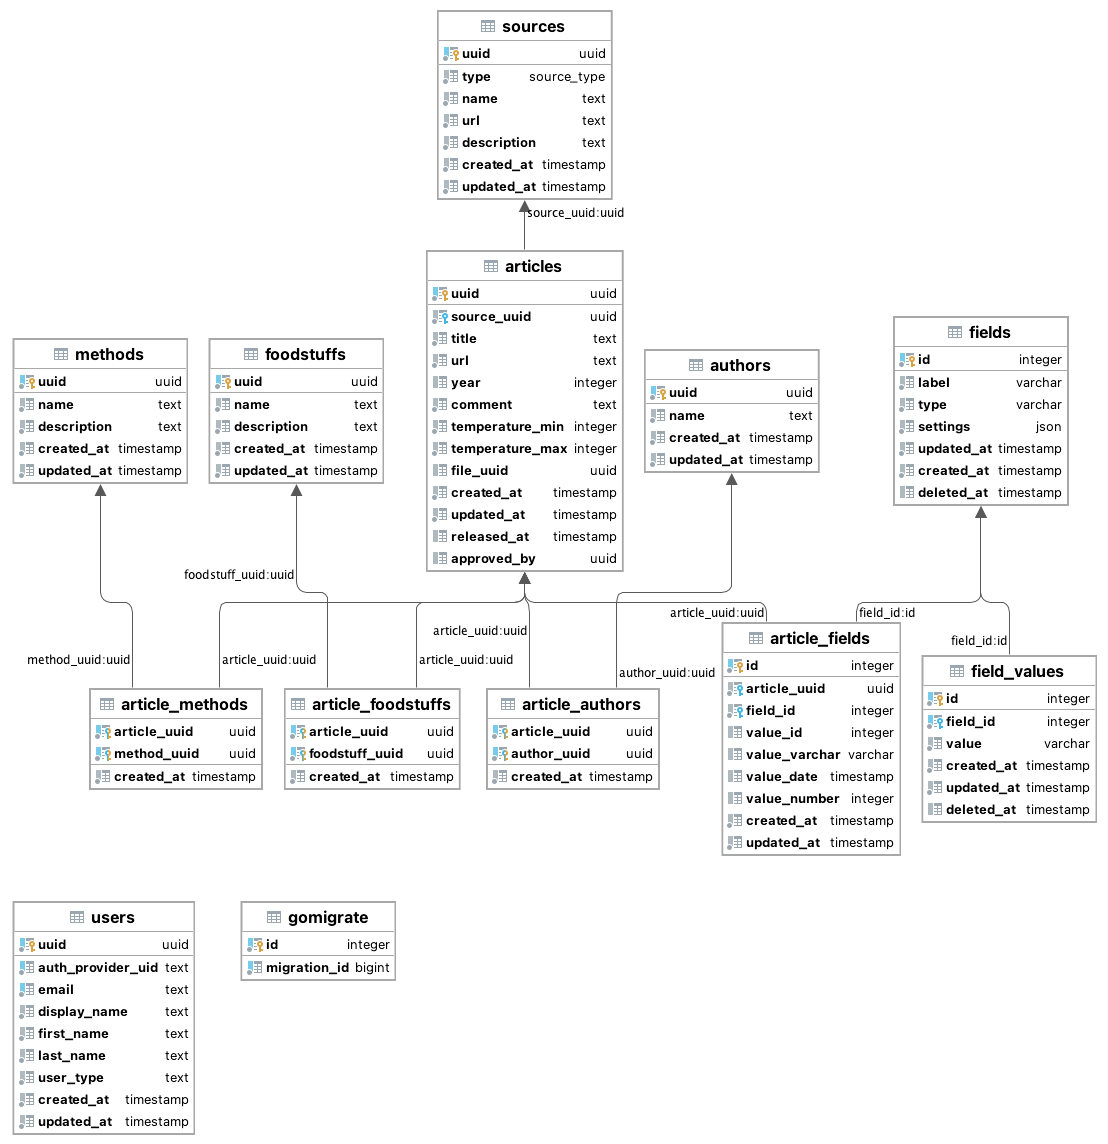
\includegraphics[width=1\textwidth]{slike/database-structure.png}
\end{center}
\caption{ Predstavitev podatkovne sheme z ER diagramom }
\label{database-diagram-er}
\end{figure}

\subsubsection{UUID}
Enoličen univerzalen identifikator - \verb=UUID= (angl. "Universally Unique Identifier") je standardna identifikacijska koda, ki se uporablja v postopku izdelave programske opreme. Uporablja se za ustvarjanje univerzalnih unikatnih identifikatorjev, ki omogočajo prepoznavanje in razlikovanje predmeta znotraj sistema ali istega predmeta v različnih kontekstih.

UUID je sestavljen iz 32 znakov (16 oktetov). Vsak znak je predstavljen v šestnajstiškem (heksadecimalnem) zapisu, kar pomeni, da je znak lahko število od \verb=0= do \verb=9=, ali pa črka od \verb=a= do \verb=f= \cite{uuid-rfc}.

Glede na ime bi lahko sklepali, da je UUID unikaten glede na čas in prostor. Vendar je končno število vseh kombinacij UUID-jev $n=2^{122}$. To pomeni, da je verjetnost, da naletimo na dva enako zgenerirana identifikatorja, zelo nizka.
Pa vendar, če zgeneriramo množico UUIDjev ($r$), kjer je število generiranih identifikatorjev večje kot največje število vseh mogočih vrednosti ($r > n$), morajo v množici obstajati duplikati. Verjetnost, da se pojavijo duplikati je mogoče natančno izračunati na podlagi rojstnodnevnega paradoksa~\cite{birthday-problem-what-is}, ki ga je leta 1932 predstavil Von Mise \cite{birthday-problem-inventor}.

\begin{izrek}
\label{iz:1}
Verjetnost unikatno generiranega UUIDja
\begin{equation}
\mathtt{\frac{n!}{n^{r}(n-r)}}
\label{eq:1}
\end{equation}
\end{izrek}

\begin{dokaz}
Število načinov, da nimamo dvojnikov je $n*(n-1)*(n-2)* …(n-(r-1))$. Kar pomeni, da je lahko prvi UUID katerakoli kombinacija od $n$ možnosti, drugi je lahko katera koli kombinacija od \verb=n=, razen prvega $(n-1)$, in tako naprej $(n-2)$... Skupno število načinov za generiranje $r$ UUID-jev je torej $n^r$, saj ima vsak, od $r$ UUIDjev $n$ različnih kombinacij.
S tem je dokaz Izreka~\ref{iz:1} zaključen.
\end{dokaz}

Če nadaljujemo računanje na podlagi rosjtnodnevnega paradoksa, pridemo do rešitve, ki nam pove, da je vrjetnost resnično majhna. Da se pojavi duplikat, bi morali vsako sekundo zgenerirati miljardo vrednosti torej 85 zaporednih let. Datoteka z zgeneriranimi UUID-ji bi bila na koncu velika $45EB$ ($45kb*1000^6$) \cite{uuid-collisions}

\subsection{Problem s poizvedbo n+1}
Pri poizvedovanju podatkov iz podatkovne baze je potrebno biti pozoren na število izvedenih klicev. Če nismo pazljivi lahko pridemo do težave s poizvedbo \verb=n+1=. Ta se zgodi, ko je ko del aplikacije izvede \verb=n= dodatnih poizvedb, da bi pridobil iste podatke, ki bi jih bilo mogoče pridobiti pri izvajanju primarne poizvedbe SQL.

Večja kot je vrednost \verb=n=, več poizvedb bo izvedenih, večji je vpliv na zmogljivost. Težava je pri izvajanju velikega števila dodatnih poizvedb, ki na splošno zahtevajo dovolj časa, da upočasnijo odzivni čas. V aplikaciji smo poskrbeli, da do težave z izvajanjem poizvedb po nepotrebnem ne bo prišlo.  



\subsection{Minio}
\label{minio-what}
Minio je samostojna rešitev za izdelavo lastne hrambe objektov. Je alternativa za bolj poznani Amazonovi storitvi AWS S3.

Programska oprema Minio je na voljo kot preprost binarni dokument in celo uradna dokumentacija kaže, da ga uporabljajo na tak način, namesto da uporabite upravitelja paketov. Seveda obstajajo Dockerjeve slike če jih želite uporabiti za zagon minio na vašem VPS.

Minio je bolj primeren za shranjevanje nestrukturiranih podatkov kot so fotografije, videoposnetki, dnevniške datoteke, varnostne kopije in slike vsebnikov / VM. Velikost predmeta se lahko giblje od nekaj KB do največ 5 TB.


\chapter{Uporaba aplikacije}
V prejšnjih poglavjih smo spoznali terminologijo, tehnologije in implementacijo teh tehnologij v našo aplikacijo. V tem poglavju pa bomo spoznali uporabo aplikacije, ki smo jo izdelali.

Aplikacija je sestavljena iz zalednega in čelnega dela. Zaledni del, je sestavljen iz večih komponent, in sledi arhitekturni postavitvi mikrostoritev. Čelni del pa je enostavna aplikacija, napisana v programskem ogrodju \verb=Vue.js=. To je del aplikacije, ki je prikazan uporabniku, zato je pomembno, da je na videz enostaven in pregleden, hkrati pa tudi hiter in funkcionalen. 


\section{Zagon aplikacije v lokalnem okolju}
Postavitev projekta je lahko včasih zelo zamudno delo, s katerim programer izgubi veliko nepotrebnega časa. 














\newpage
\chapter{Predstavitev Aplikacije}
V prejšnjem poglavju smo spoznali posamezne tehnologije in orodja, ki smo jih uporabili za izvedbo naše aplikacije. V naslednjem sklopu pa bomo spoznali kako smo omenjene tehnologije in orodja uporabili. 

Aplikacija je sestavljena iz zalednega in čelnega dela. Zaledni del, je sestavljen iz večih komponent, in sledi arhitekturni postavitvi mikrostoritev. Čelni del pa je enostavna aplikacija, napisana v programskem ogrodju \verb=vue.js=. To je del aplikacije, ki je prikazan uporabniku, zato je pomembno, da je na videz enostaven in pregleden, hkrati pa tudi hiter in funkcionalen. 



\section{Postavitev projekta v lokalnem okolju}

Namen dobrega razvojnega okolja je, da ima uporabnik (programer), možnost rekonstruiranje celotnega razvojnega okolja z čim manj vloženega truda. To mu zagotavlja, da projekt povrne v stanje, ki ga imajo vsi ostali programerji, in s tem izniči velik delež samostojne napake, ki se lahko zgodi pri programiranju programske opreme. Velikokrat se lahko zgodi da je težava v infrastruktuiri, zaradi napačne postavitve samega projekta. Tej težavi smo se hoteli izogniti z pravilno postavitvijo projekta.

Za naš projekt, smo se odločili za uporabo vsebovalnikov (angl. containers). Sama implementacija je narejena z orodjem \verb=Docker=. Izvedba je nostavna in je definirana z konfiguracijskimi datotekami. Za zagon projekta je potrebno imeti prednameščeni orodji \verb=Docker= in \verb=Git=.

Z uporabo orodja \verb=Git=, je potrebno prenesti celoten projekt na razvijalčev računalnik. Razvijalec mora imeti dostop do repozitorija, ki je na voljo na platformi \verb=GitHub=. Ko ima razvijalec vse potrebne dostope in pravice, mu je omogočen prenos vseh datotek na njegov računalnik. 
To stori z ukazom \ref{lst:git-clone}.

\begin{lstlisting}[language=bash,style=mystyle,caption={Uporaba orodja Git, za prenos projekta},label=lst:git-clone]
$ git clone git@github.com:marolt/diploma.git
\end{lstlisting}

\subsection{Postavitev zalednega dela aplikacije}
Zagon aplikacje je odvisen kar od nekaj komponent. Za medsebojno delovanje in odvisnost vsebnikov poskrbi orodje \verb=docker-compose=. Docker Compose je ogrodje razvito okrog Docker sistema, ki nam omogoča enostavno orkestracijo vsebovalnikov. Z definiranjem konfiguracijske datoteke \verb=docker-compose.yml= (Koda \ref{lst:dco-snipet}), smo nastavili povezave med posameznimi storitvami, kakšna vrsta omrežja naj bo uporabljena, spremeljivke okolja, katero sliko vsebovalnika naj posamezna storitev uporabi, katera vrata naj odpre na gostitelja, in se ostale stvari, ki so potrebne za postavitev celotne arhitekture.

Za vsako storitev je definiran vsebovalnik, ki ima definirano katero sliko naj uporabi. Za zaganjanje programske kode v go programskem jeziku, medtem ko smo aplikacijo razvijali, smo zraven osnovne slike pripeli še dodatno orodje za osveževanje kode \ref{lst:dcf-snipet}.

\begin{lstlisting}[style=mystyle,caption={Dockerfile datoteka za razvijanje Go programske opreme},label=lst:dcf-snipet]
FROM golang:1.17
RUN go get github.com/cespare/reflex
COPY reflex.conf /
COPY run.sh /
ENTRYPOINT ["reflex", "-c", "/reflex.conf"]
\end{lstlisting}

Uporabili smo osnovno sliko $\verb=golang:1.17=$, ki je uradna slika iz strani razvijalcev programskega jezika Go. Naslednji ukaz $\verb=RUN=$ zažene ukaz za namestitev orodja $\verb=reflex=$, ki omogoča sprotno osveževanje kode med samim razvojem v programskem jeziku Go. Ukaz $\verb=COPY=$ prekopira datoteko $\verb=reflex.conf=$ in $\verb=run.sh=$ iz gostiteljevega datotečnega sistema. Zadnji ukaz v datoteki, $\verb=ENTRYPOINT=$ pa zažene ukaz $\verb=reflex=$ z dodatnimi parametri, ki definirajo konfiguracijko datoteko. Ta ukaz se bo vedno zagnal ob vsakem zagonu vsebovalnika.

\begin{lstlisting}[style=mystyle,caption={Izsek konfiguracijske datoteke docker-compose.yml},label=lst:dco-snipet]
version: '3'
services:
  db:
    image: postgres:9.6.23
    env_file:
      - docker.env
    ports:
      - "5433:5432"
    volumes:
      - postgresql-data:/var/lib/postgresql/data/
  app:
    build:
      context: docker/app
    volumes:
      - .:/src
    working_dir: /src/articles
    ports:
      - "3000:80"
    env_file:
      - .env
    depends_on:
      - minio
      - db
  minio:
    image: minio/minio
    volumes:
      - minio-volume:/export
    ports:
      - "9000:9000"
    command: server /export
volumes:
...
\end{lstlisting}
V izseku kode (\ref{lst:dco-snipet}) lahko vidimo, kako so posamezni vsebovalniki definirani v datoteki docker-compose.yml. Razvidna je tudi njihova medsebojna odvisnost, kot naprimer za delovanje vsebovalnika $app$ je potrebno, da sta dosegljiva tudi ostala dva vsebovalnika ($db$ in $minio$).

Da je delo na projektu še bolj enostavno smo ukaze ovili z orodjem \verb=Makefile=. To orodje nam omogoča, definiranje opravil, ki zaženejo sklop ukazov (ali skripto). 

\begin{lstlisting}[language=bash,style=mystyle]
$ make start
\end{lstlisting}

Zgornji ukaz poskrbi za postavitev našega projekta v okolju za razvijanje. V ozadju se izvede niz ukazov, ki zagotovijo, da so vse storitve na voljo. To lahko preverimo z ukazon $\verb=docker-compose ps=$ (Koda \ref{lst:running-containers}), kjer se izpiše aktivno stanje zagnanih vsebovalnikov. Iz izpisanega, lahko razberemo, da se ob postavitvi projekta zažene devet vsebovalnikov.  

\begin{lstlisting}[language=bash,style=mystyle,caption={Prikaz zagnanih vsebovalnikov},label=lst:running-containers]
$ docker-compose ps

Name           Command                State  Ports
------------------------------------------------------------
d_web_1        /run.sh.                 Up   :80->80/tcp
d_app_1        reflex -c /reflex.conf   Up   :3002->80/tcp
d_users_1      reflex -c /reflex.conf   Up   :3001->80/tcp 
d_firestore_1  dockerize -template=/... Up   :9099->9099/tcp             
                                             8787/tcp
d_minio_1      /usr/bin/docker-entry... Up   9000/tcp     
d_memcached_1  docker-entrypoint.sh ... Up   11211/tcp     
d_postgres_1   docker-entrypoint.sh ... Up   :5433->5432/tcp       
d_trace_1      /go/bin/all-in-one-linux Up   14250/tcp 
                                            :14268->14268/tcp
                                            :16686->16686/tcp
                                            5775/udp,5778/tcp 
                                            6831/udp,6832/udp   
d_teus_1       /bin/prometheus --con... Up  9090/tcp     
\end{lstlisting}

Za razvojno okolje, nekaterih storitev ni smiselno izolirati na nivoju infrastrukture. V našem primeru si naše storitve delijo skupni vsebovalnik za podatkovno bazo, in s tem prihranimo na hitrosti lokalnega razvoja. Razvoj aplikacije je v našem primeru enostavnejši in preglednejši, vendar moramo biti med razvojem pazljivi, da ohranimo medsebojno neodvisnost samih storitev. 

Za lažjo predstavitev, nam je na voljo diagram celotne arhitekure prikazan na sliki \ref{final-arch}

\begin{figure}[h]
\begin{center}
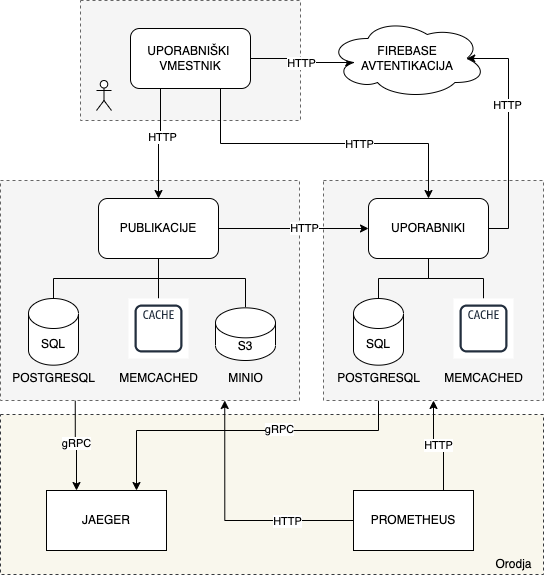
\includegraphics[width=0.75\textwidth]{slike/arch-done.png}
\end{center}
\caption{ Arhitektura projekta predstavljena z diagramom }
\label{final-arch}
\end{figure}

\subsection{Postavitev čelnega dela aplikacije}
Čelni sistem uporablja $\verb=javaScript=$ ogrodje \verb=vue.js=. Ogrodje je odvisno od \verb=node.js= programskih datotek, zatorej moramo v sliko vsebovalnika namestiti potrebne stvari za delovanje tega ogrodja. 

V namšem primeru (Koda: \ref{lst:dcf-node}) uporabimo pred definirano sliko \\ \texttt{node:17.3.0-alpine3.14}, ki že ima nameščena orodja kot so \texttt{node.js} in upravljec paketkov \texttt{npm}. Ker je vmestnik uporabljen v razvojnem okolju, definiramo vrednost \texttt{NODE\_ENV} na \texttt{development}. Skripta \texttt{run.sh} je skopirana v sliko z dodatnimi pravicami, za zagon. Na koncu se skipto sproži v izvajanje.

\begin{lstlisting}[,style=mystyle,caption={Dockerfile datoteka za razvijanje Vue aplikacije},label=lst:dcf-node]
FROM node:17.3.0-alpine3.14

ENV NODE_ENV development

ADD start.sh /
RUN chmod +x /start.sh

CMD ["/run.sh"]
\end{lstlisting}

V datoteki $start.sh$ (\ref{lst:dcf-run}) so navedeni ukazi, ki se zgodijo ob vsakem zagonu vsebovalnika. Komanda \texttt{npm install} namesti vse potrebne knjižnjice, ki jih v aplikaciji uporabljamo. Komanda \texttt{npm serve} pa zažene spletni strežnik, ki streže vsebino aplikacije iz trenutnega direktorija.

\begin{lstlisting}[language=bash,style=mystyle,caption={Ukazna datoteka, ki nasneme potrebne knjižnice in streže aplikacijo},label=lst:dcf-run]
set -e

npm install
npm serve
\end{lstlisting}

Pomembno je tudi poudariti, da je aplikacija enostranska (angl. single-page), kar pomeni, da deluje znotraj brskalnika in ne potrebuje ponovnega nalaganja strani med svojim delovanjem. Je le ena sama stran, ki jo obiščemo in na kateri se nato naloži vso ostalo vsebino s pomočjo JavaScripta.

Kot je razvidno iz prikaza zagnanih vsebovalnikov (Koda: \ref{lst:running-containers}), ima čelni del odprta vrata 80, kar pomeni, da je stran dostopna na lokalnem spletnem naslovu \url{http://localhost:80/}. 



\section{Predstavitev uporabniškega vmestnika}
V tem delu bomo spoznali kako je zasnovan čelni del naše aplikacije in kako komunicira z zalednim sistemom. Pri razvoju tega dela aplikacije je potrebno biti pozoren na kar nekaj stvari, kot je naprimer zasnova na videz lepega, vendar uporabnega grafičnega vmestnika, preko katerega uporabnik varno komunicira z našim zalednim sistemom. Med samo uporabo in komunikacijo ne smemo pozabiti na ustrezno prikazovanje napak uporabniku, da sam uporabnik ve kdaj je do napake prišlo in kako jo odpraviti.

Čelni del aplikacije uporablja ogrodje \verb=Vue.js= (\ref{vue-js-section}), ki je zelo enostavno \verb=JavaScript= ogrodje z številnimi orodji in knjižnicami, s katerimi si poenostavimo in pohitrimo razvoj. Knjižnice, ki jih aplikacija potrebuje, so navedene v datoteki \verb=package.js= (glej kodo \ref{lst:pkg-snippet}). V omenjeni datoteki so navedeni tudi ukazi, s katerimi prožimo določene akcije, kot so gradnja statičnih paketov, postavitev spletnega strežnika za streženje datotek in gradnja CSS datotek z pomočjo knjižnice \verb=tailwind=. Za nadzor nad uporabljenimi knjižnicami skrbi orodje \verb=NPM= (angl. Node Package Manager).

\begin{lstlisting}[language=php, style=mystyle,caption={Izsek naštetih knjižnic in ukazov v datoteki package.json},label=lst:pkg-snippet]
{
  "name": "diploma",
  "version": "1.0.0",
  "private": true,
  "scripts": {
    "serve": "vue-cli-service serve",
    "build": "vue-cli-service build",
    "lint": "vue-cli-service lint",
    "build:tailwind": "npx tailwindcss ...",
    "install:clean": "rm -rf node_modules/ ..."
  },
  "dependencies": {
    "@fortawesome/fontawesome-free": "^5.15.4",
    "@tailwindcss/forms": "^0.3.4",
    "@vueform/multiselect": "^2.2.1",
    "@vueform/slider": "^2.0.8",
    "core-js": "^3.19.1",
    "firebase": "^9.3.0",
    "jsonwebtoken": "^8.5.1",
    "litepie-datepicker": "^1.0.14",
    "lodash": "^4.17.21",
    "moment-timezone": "^0.5.34",
    "register-service-worker": "^1.7.1",
    "superagent": "^6.1.0",
    "v-tooltip": "^4.0.0-beta.2",
    "vue": "^3.2.21",
    "vue-router": "^4.0.0-0",
    "vue-toast-notification": "^2.0.1"
  },
  "devDependencies": {
     ...
    "sass": "^1.32.5",
    "sass-loader": "^10.1.1",
    "tailwindcss": "^2.2.19"
  }
}

\end{lstlisting}

\section{Pozdravna stran}
Ob obisku spletnega mesta \url{http://localhost} se odpre \sn{Pozdravna stran} (Slika \ref{landing-page}). Stran je namenjena vsem uporabnikom, da se seznanijo z aplikacijo. Vsebuje povezave na zunanje vire, kjer lahko uporabnik pridobi koristne informacije o živilih. 

S klikom na gumb \sn{VSTOPI V APLIKACIJO}, je uporabnik usmerjen v aplikacijo. Če, kot uporabnik ni prijavljen, se mu odpre stran za prijavo (\ref{sign-in-page}). V primeru, da je že prijavljen, se pravi, ima tekočo sejo, pa se mu odpre domača stran znotraj aplikacije, kjer lahko uporabnik prebera in izvaja filtre nad vnešenimi publikacijami (\ref{filters-page}).

\begin{figure}[h]
\begin{center}
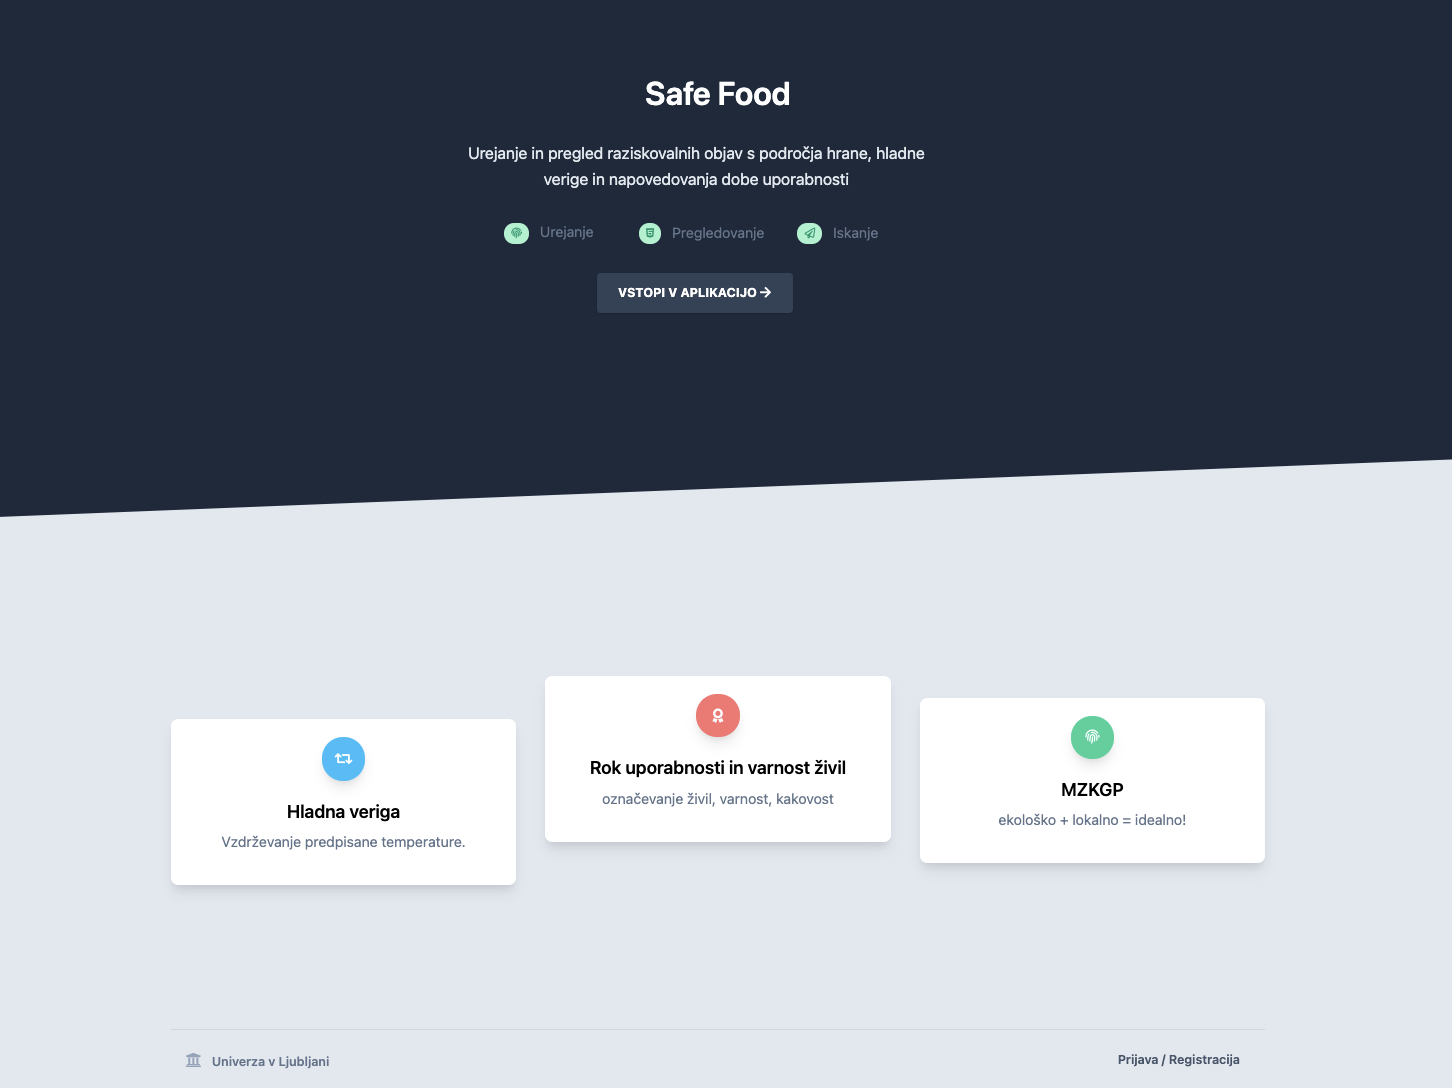
\includegraphics[width=1\textwidth]{slike/landing-page.png}
\end{center}
\caption{ Pozdravna stran }
\label{landing-page}
\end{figure}


\section{Stran za registracijo}
\label{registration-page}
Za uporabo aplikacije je potrebna registracija uporabnika. Uporabnikom, ki se niso registrirani v aplikacijo, je dana možnost, da si kreirajo račun (glej sliko \ref{signup-form}).

\begin{figure}[h]
\begin{center}
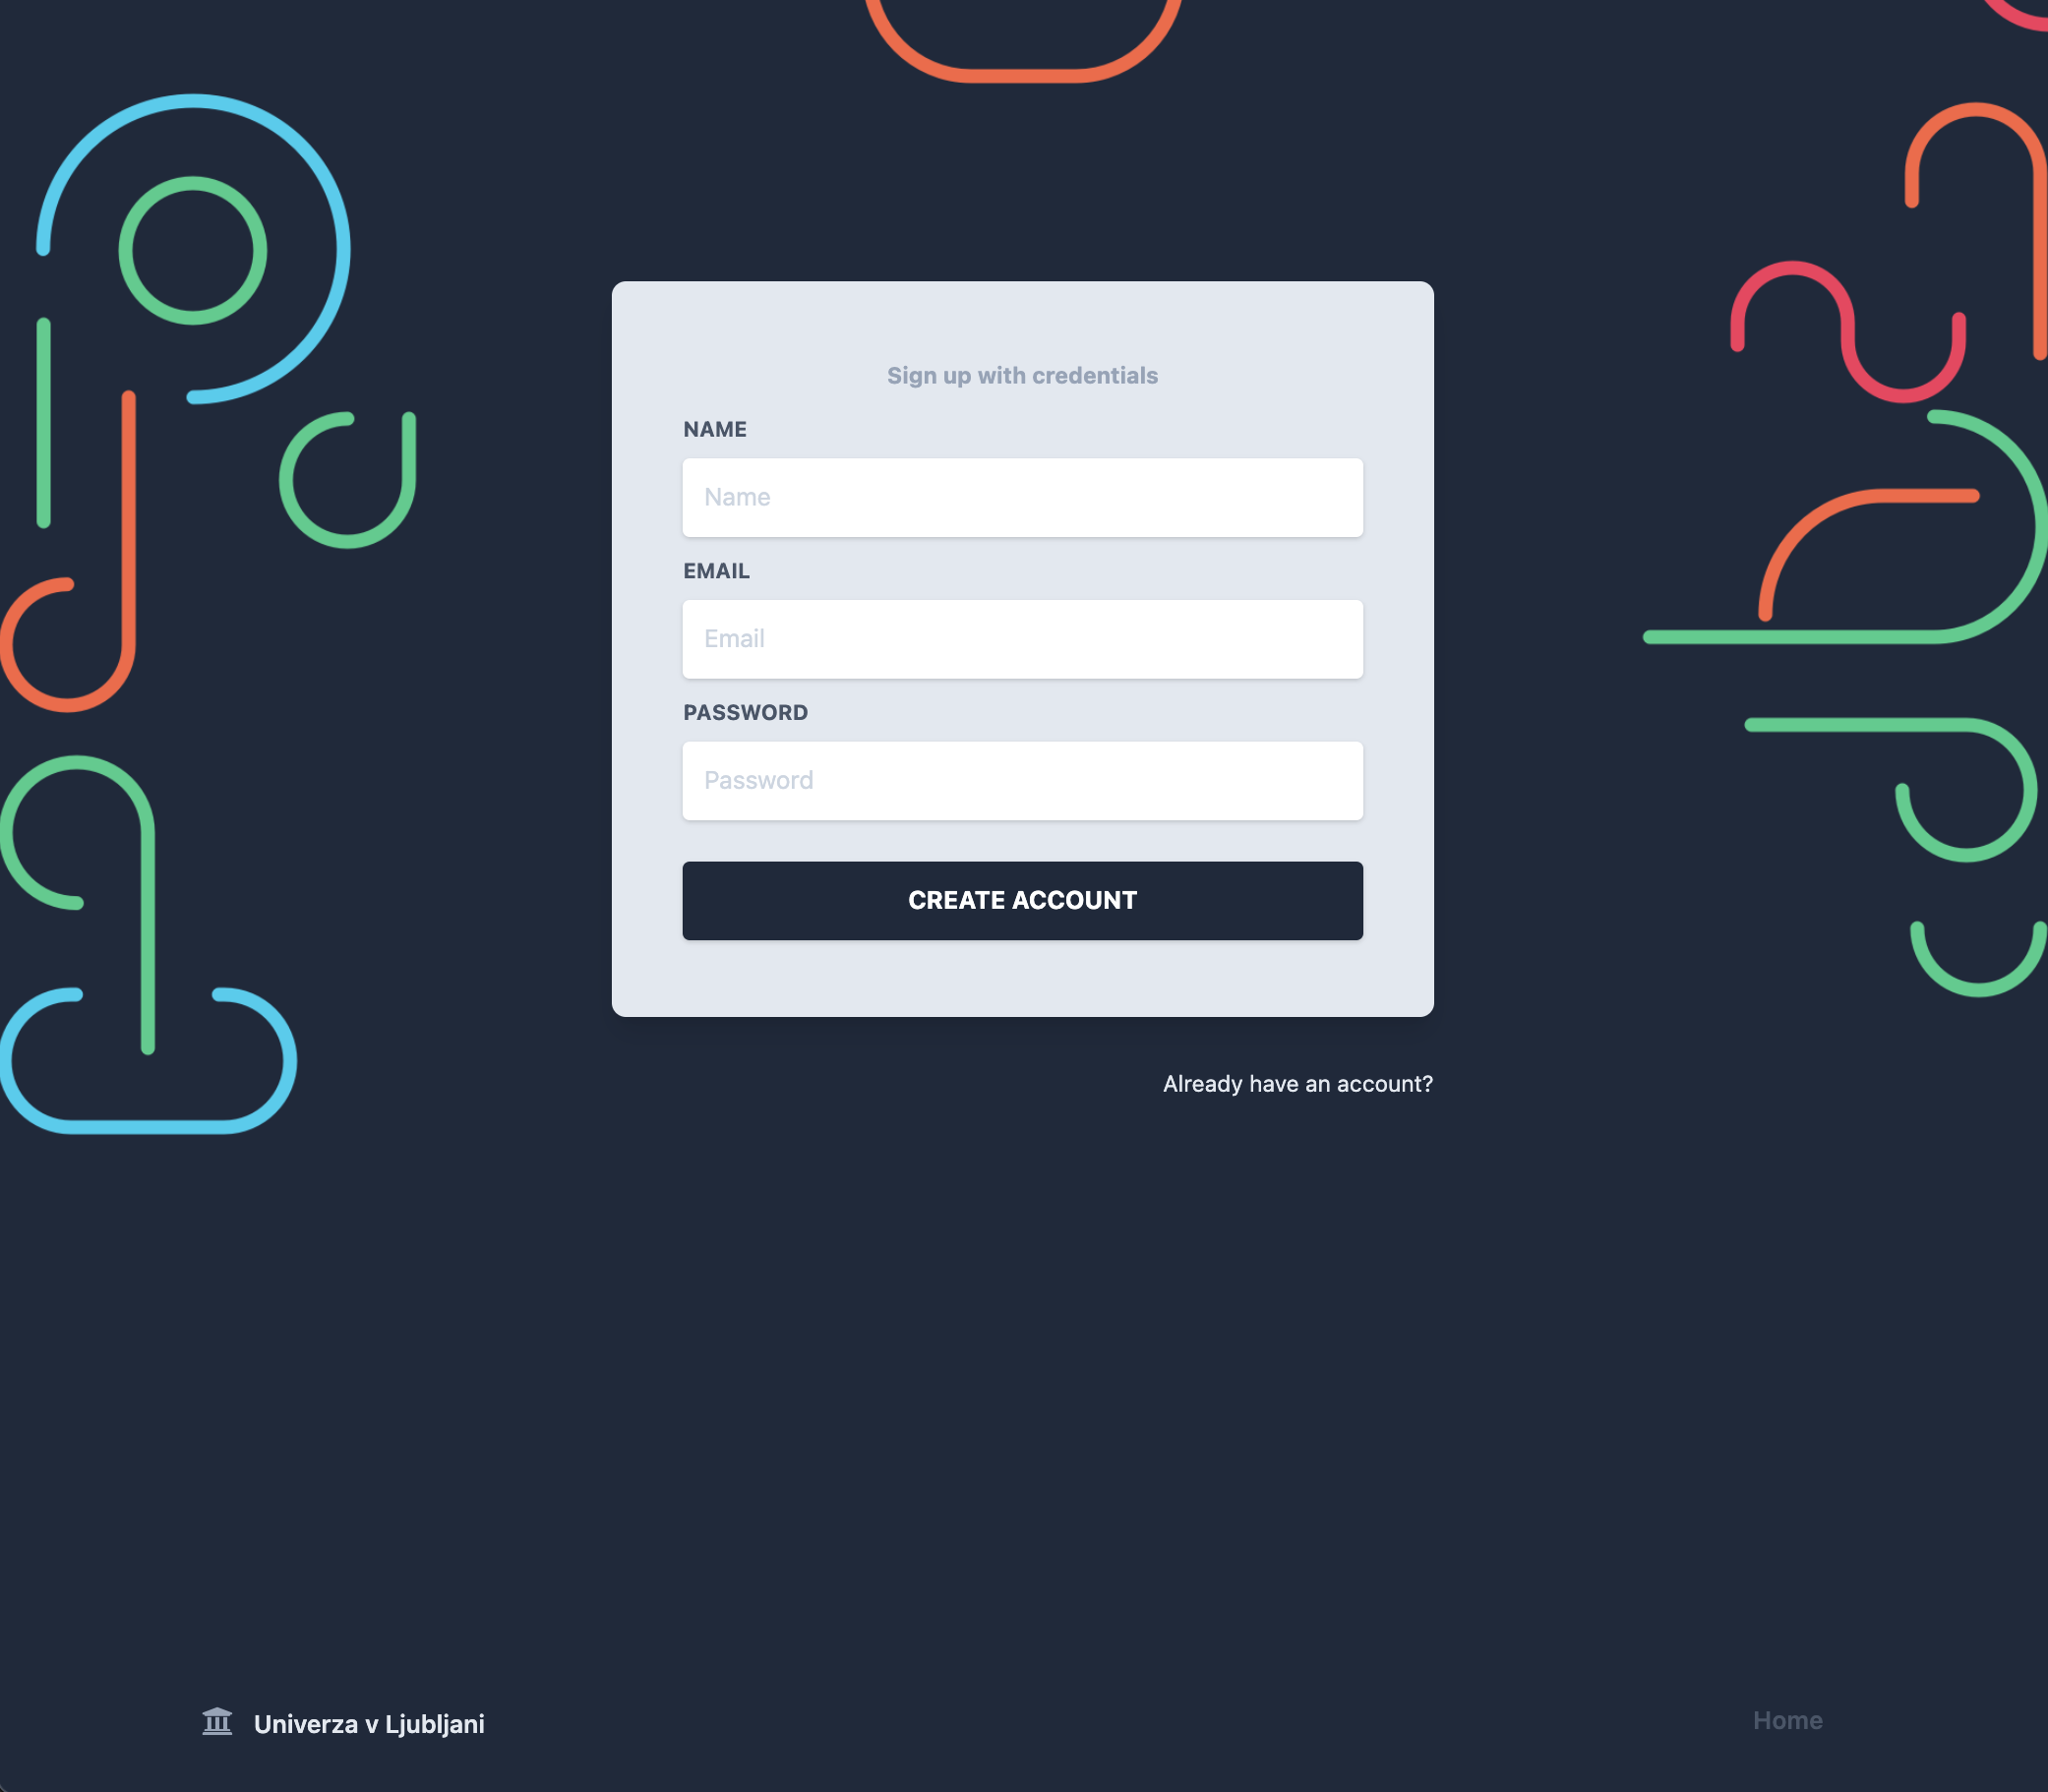
\includegraphics[width=1\textwidth]{slike/signup.png}
\end{center}
\caption{ Registracijska forma }
\label{signup-form}
\end{figure}

Uporabniško ime mora ustrezati definiranemu formatu, ki je določen kot regularni izraz in mora vsebovati vsaj tri znake (\ref{lst:validation}). V primeru, da uporabnik vnese napačno uporabniško ime ali geslo, se na vrhu vnosnih polj izpiše ustrezno opozorilo o napaki. Validacija se izvaja na zalednem iz čelnem delu.

\begin{figure}[ht]
\begin{center}
\begin{lstlisting}[language=java, style=mystyle,caption={Primer validacijske funkcije za preverjanje uporabniškega imena z uporabo regularnega izraza},label=lst:validation]
function validateUsername(uname) {
  /*
    Uporabnisko ime, ne sme biti krajse od treh znakov
  */
  if(uname.length < 3) {
    return false;
  }

  /* 
    Vsebuje lahko le: 
    - male crke (a-z) 
    - stevilke (0-9)
    - pike (.)
    - podcrtaje (_)
  */
  const match = /^[a-z0-9_\.]+$/.exec(uname);
  
  // veljavno ali ne
  return Boolean(rezultat);
}
\end{lstlisting}
\end{center}
\end{figure}

Ob registraciji, uporabnik na vnešen elektronski naslov prejme novo sporočilo za potrditev uporabniskega računa. To sporočilo je namenjeno zagotavljanju verodostonjosti uporabnika, s potrditvenim sporočilom. V primeru, da uporabnik ne potrdi njegovega poštnega predala v roku enega dneva, mu je dostop do aplikacije onemogocen, vse dokler uporabik ne potrdi računa.

Nepotrjen uporabnik nima dostopa do dela aplikacije, kjer so prikazane publikacije. Pokaže se mu le stran z navodili, kako potrditi poštni naslov. V primeru, da uporabnik ni prejel potrditevega sporočila, lahko klikne na gumb, in sproži ponovno pošiljanje potrditevega sporocil. Sporočilo bo bilo ponovno zgenerirano le v primeru, da je minila vsaj ena ura od zadnjega poizkusa pošiljanja tega sporočila.

Vsak uporabnik je ob registraciji le navaden uporabnik. Vlogo uporabnika lahko spremeni le administrator, v administracijskem delu aplikacije. O tem bomo govorili v sekciji "Administracija uporabnikov" (\ref{administracija-uporabnikov}).

V elektronskem sporočilu, ki ga uporabnik prejme na svoj poštni naslov, je navedena povezava do naše aplikacije. Generirana povezava vsebuje parameter \verb="method"=, ki nam pove, katera akcija se mora izvesti, ko uporabnik odpre stran. Vue komponenta, prebere url parameter, in glede na prebran parameter sproži ustrezno akcijo na autentikacijski servis. Implementirane imamo akcijo za ponastavitev gesla in pa akcijo za potrditev poštnega naslova (\ref{auth-methods}).

\begin{figure}[h]
\begin{center}
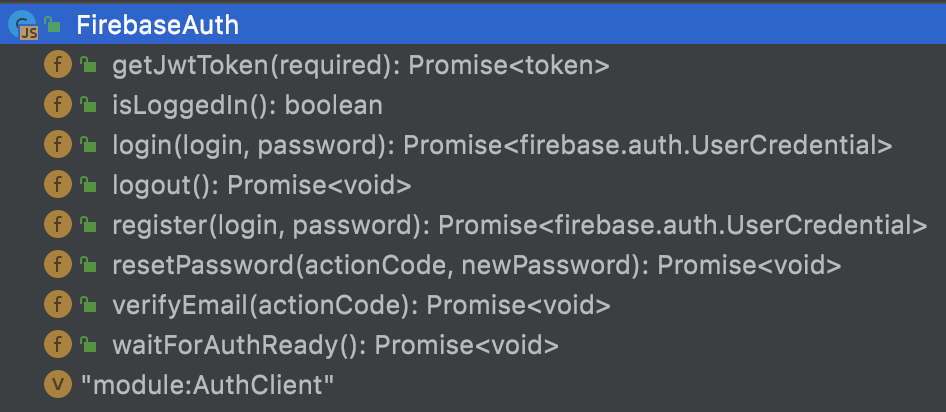
\includegraphics[width=1\textwidth]{slike/firebase_auth.png}
\end{center}
\caption{ Prikaz metod za implementacijo avtentikacijskega servisa }
\label{auth-methods}
\end{figure}

V primeru, da je uporabniški račun uspešno potrjen, je uporabnik preusmerjen na zaćetno stran aplikacije, kjer lahko izvaja iskanje nad vnešenimi publikacijami. Zgodi pa se lahko tudi, da postni naslov ni uspešno potrjen (glej kodo \ref{lst:verify-username}). Do slednjega primera pa lahko pride v naslednjih primerih:
\begin{myitemize}
  \item potrditvena koda je potekla
  \item neveljavna potrditvena koda
  \item izbrisan uporabniški račun
  \item onemogočen uporabniški račun
\end{myitemize}

\begin{lstlisting}[language=bash, style=mystyle,caption={Primer kode, za verificiranje uporabnika},label=lst:verify-username]
  mounted() {
    // http://localhost:8080/auth/firebase?mode=resetPassword&oobCode={code}
    this.mode = queryParams.mode;
    this.oobCode = queryParams.oobCode;

    if (this.mode === "verifyEmail") {
      verifyAccount(this.oobCode).then(() => {
          this.$toast.success("Email verified");
          this.$router.push("home");
        }, (error) => {
          switch (error.code) {
            case 'auth/expired-action-code':
              this.$toast.error('Code expired!')
              break;
            case 'auth/invalid-action-code':
              this.$toast.error('The code is not valid.')
              break
            case 'auth/user-disabled':
              this.$toast.error('Account is disabled, please contact us at support@example.com')
              break
            case 'auth/user-not-found':
              this.$toast.error('Your account has been removed')
              break
            default:
              this.$toast.error('Email verification failed!')
          }
        });
    }
  }
\end{lstlisting}



\section{Prijavna stran}
\label{sign-in-page}
Uporabnik z obstoječim uporabniškim računom se lahko prijavi z uporabniškim imenom in geslom. V primeru, da je geslo pozabil, lahko s klikom na \sn{Pozabljeno geslo} nadaljuje na stran, kjer se mu odpre stran, za ponastavitev gesla (\ref{forgotten-form}). Implementirali smo tudi varnostni mehanizem, ki preprečuje uporabniku ugibati gesla. V primeru, da je uporabnik poizkusil že več kot dvajeset kombinacij gesla, se mu prijavo upočasni na deset na minuto. 
\begin{figure}[h]
\begin{center}
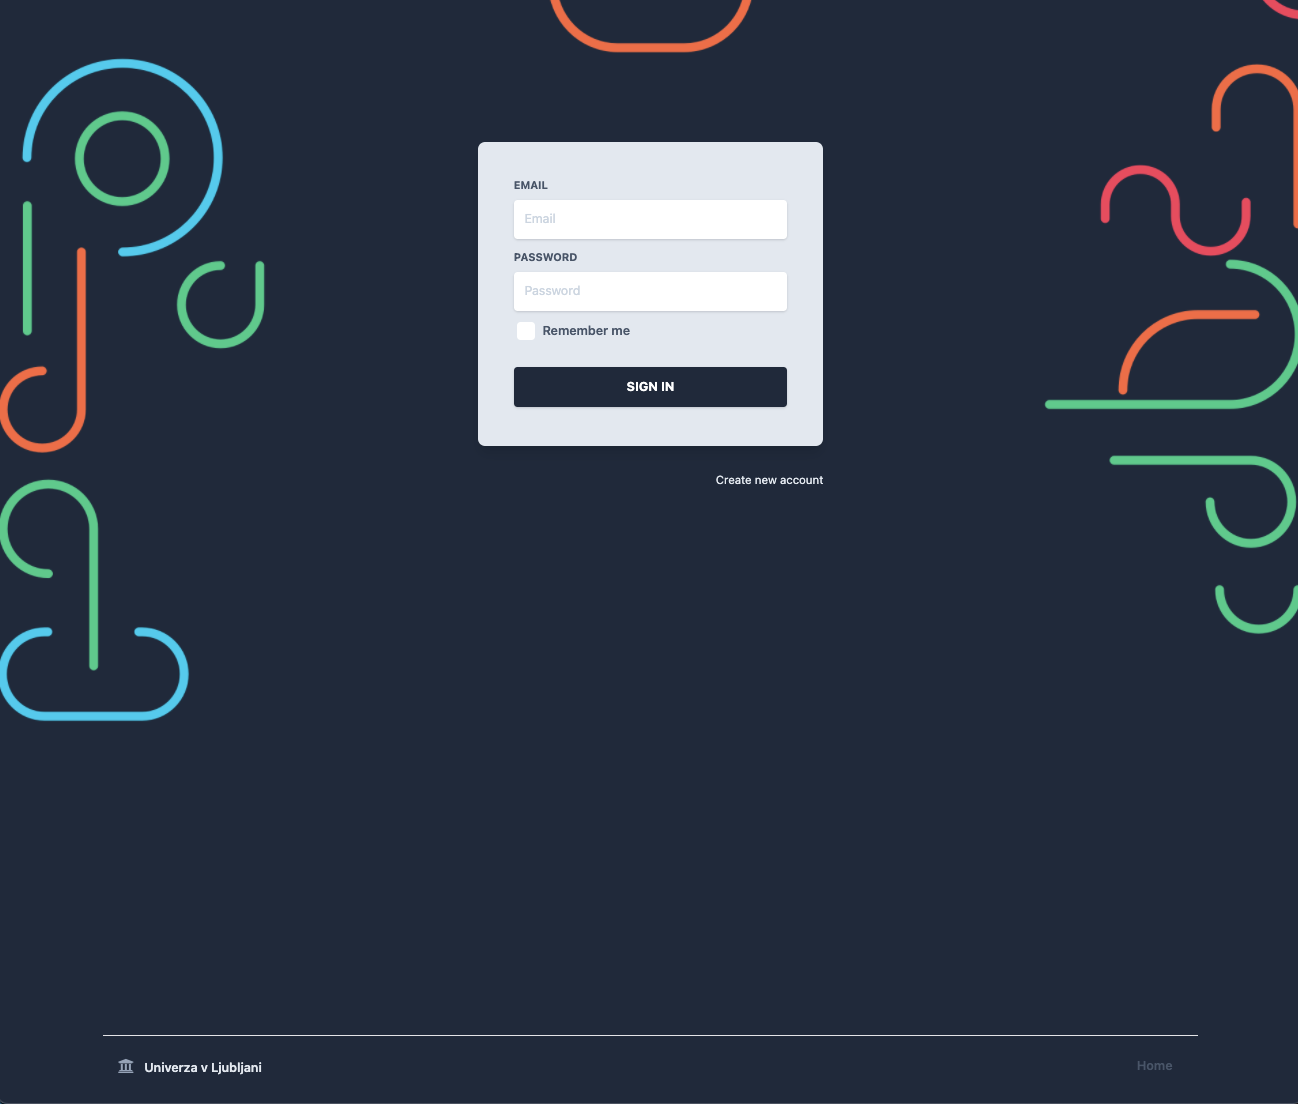
\includegraphics[width=1\textwidth]{slike/login-page.png}
\end{center}
\caption{ Prijavna stran }
\label{login-form}
\end{figure}

\section{Pozabljeno geslo}
\label{forgotten-form}
Uporabnik ima možnost obnovitve pozabljenega gesla. S klikom na gumb, se mu odpre pojavno okno, kamor vnese poštni naslov, s katerim je uporabnik identificiran v aplikacijo. Na vnešen poštni naslov, se pošlje sporočilo, ki zajema unikatno zgeneriran URL, preko katerega ima uporabnik možnost določitve novega gesla za njegov račun. 

Ob uspešni nastavitvi gesla, je uporabik preusmerjen na prijavno stran, kjer se mora prijaviti z geslom, ki ga je pravkar nastavil.

\begin{figure}[h]
\begin{center}
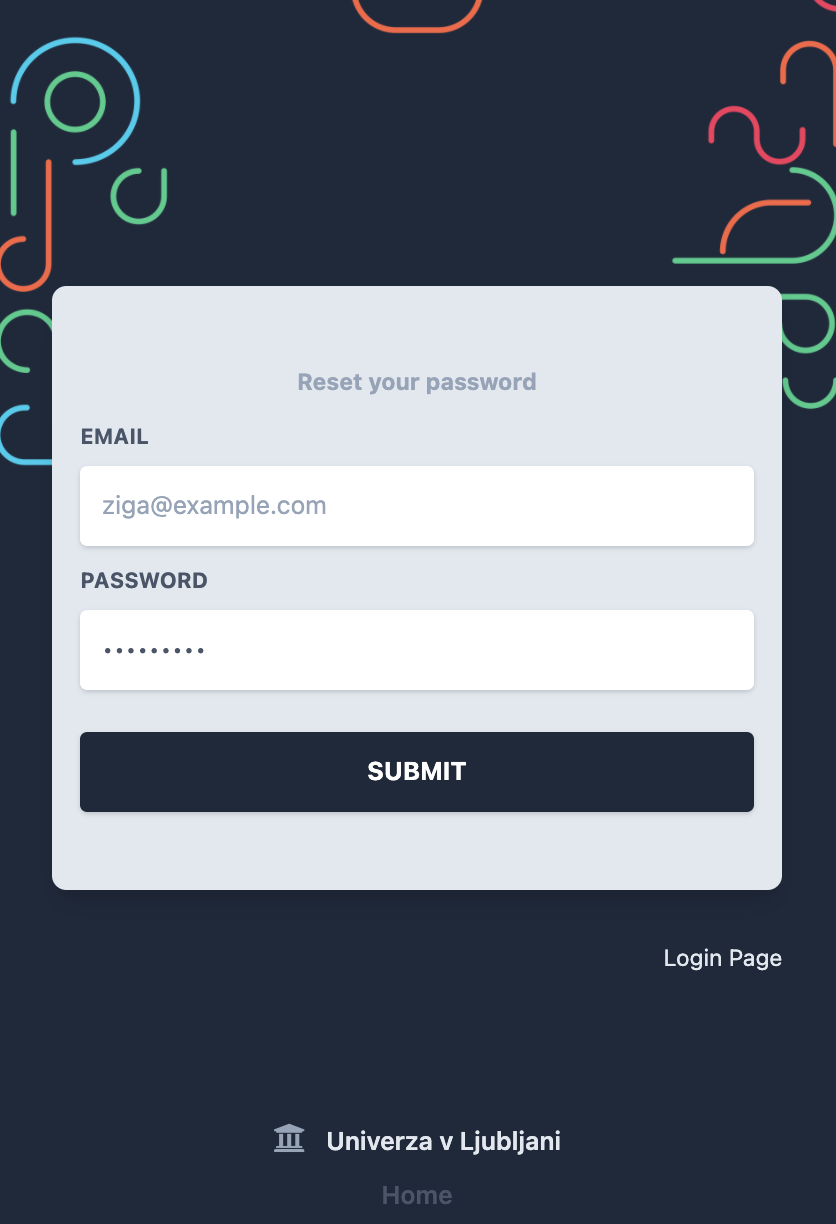
\includegraphics[width=0.5\textwidth]{slike/reset_password.png}
\end{center}
\caption{ Vnos novega gesla }
\label{password-reset-form}
\end{figure}

\section{Urejanje uporabnikov}
\label{administracija-uporabnikov}
Administratorjem je na voljo pregled in urejanje uporabnikov. Na strani \sn{Users List} (glej sliko \ref{users-list-page}), so našteti vsi uporabniki, ki so registrirani v aplikacijo. Administrator ima možnost urejanje le teh. Z klikom na ikono za smeti, je administratorju na voljo onemogočiti račun uporabnika. Z klikom na ikono za urajenje pa se odpre stran za urajanje izbranega uporabnika. Na voljo je spreminjanje uporabniškega imena, poštnega naslova in ostalih informacij uporabnika, kot so ime in priimek. Administratorju je tudi na voljo spreminjanje vrste uporabnika, torej lahko nekemu uporabniku doda pravice za urednika, ga dodeli kot administratorja, ali pa kot navadnega uporabnika, ki lahko prebira vnešene publikacije.

\begin{figure}[h]
\begin{center}
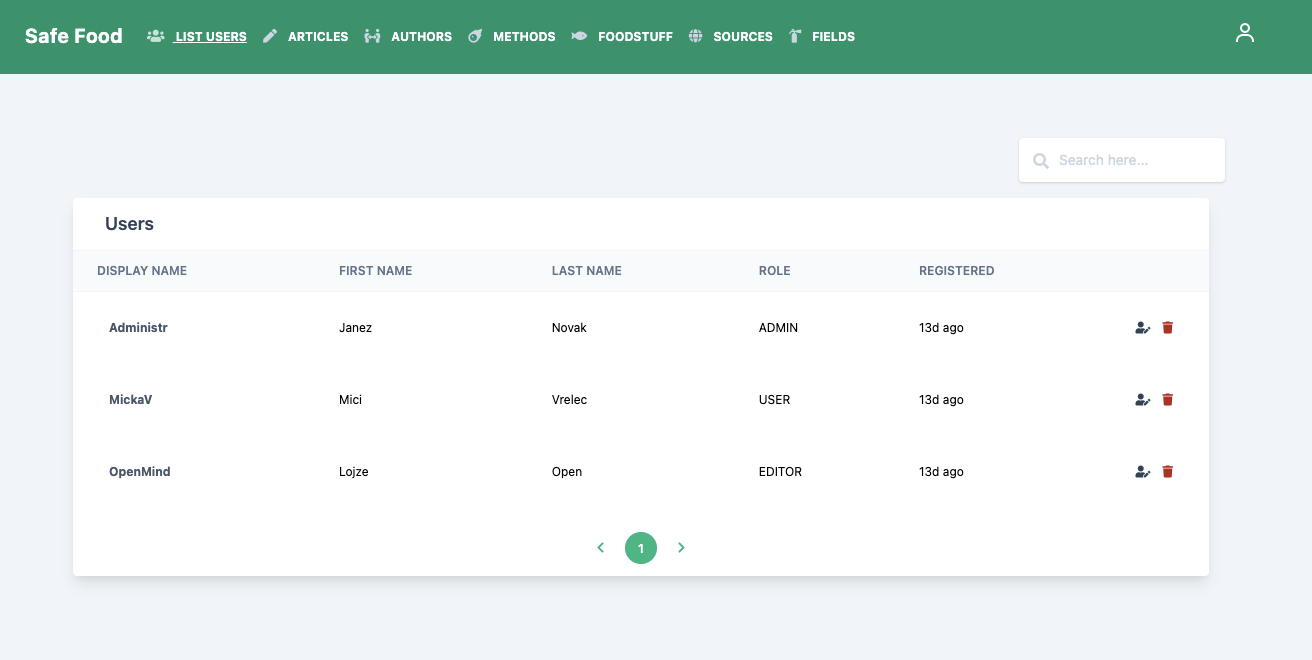
\includegraphics[width=1\textwidth]{slike/users-list.png}
\end{center}
\caption{ Stran za urejanje uporabnikov }
\label{users-list-page}
\end{figure}


\section{Razvoj dinamičnega dodajanja podatkov}
Za potrebe aplikacije smo razvili popolnoma dinamičen način za dodajanje posameznih podatkov. Uporabnik z uporabniškimi pravicami \sn{urednik}, ali \sn{administrator}, ima možnost definiranja novih parametrov za publicitacijo. Nove parametre lahko definira na strani \sn{Fields} (glej sliko \ref{fields-list}). 

\begin{figure}[h]
\begin{center}
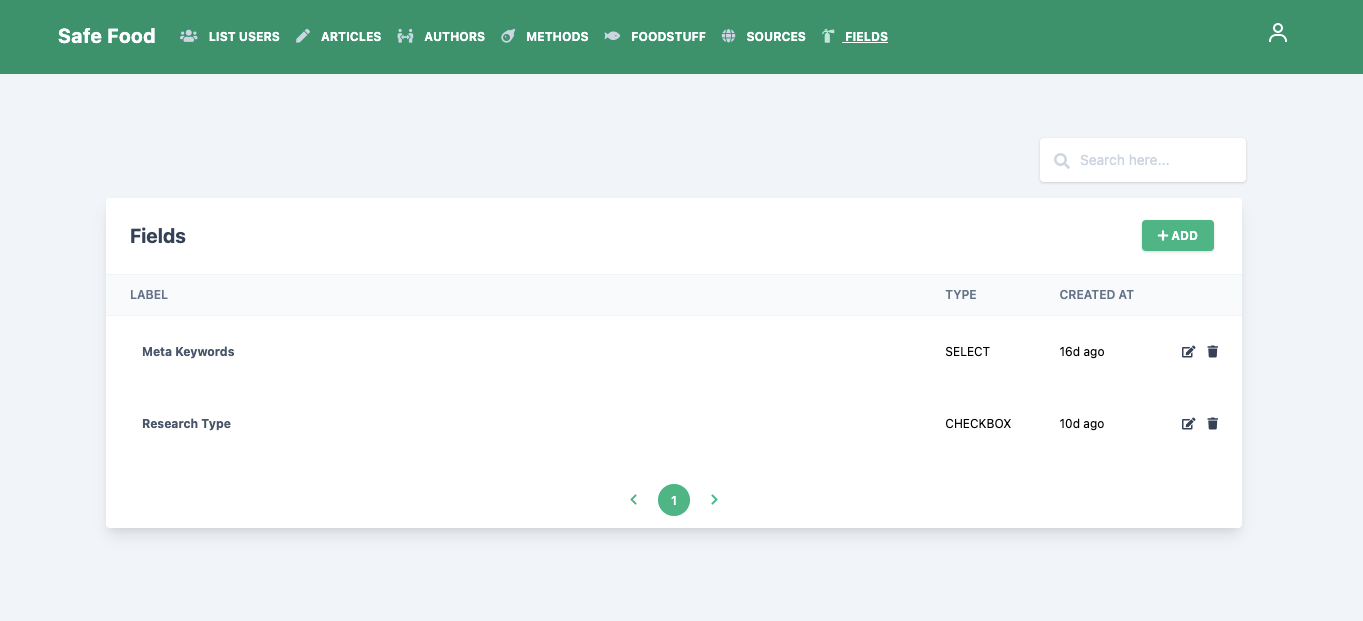
\includegraphics[width=1\textwidth]{slike/fields-list.png}
\end{center}
\caption{ Stran za prikaz in urejanje dinamičnih parametrov }
\label{fields-list}
\end{figure}

Namen dinamičnih parametrov je, da je uporabniku omogočeno dodajanje novih parametrov za publikacijo, podatkov, ki še nisi bili definirani v sistem. Te paremetre lahko uporabnik dodaja, ureja in briše medtem ko ureja publikacijo (glej sliko \ref{field-usage-example-select}). Za vsak dinamično definiran parameter, je uporabniku avtomatično omogočeno filtriranje po teh podatkih. 

\begin{figure}[h]
\begin{center}
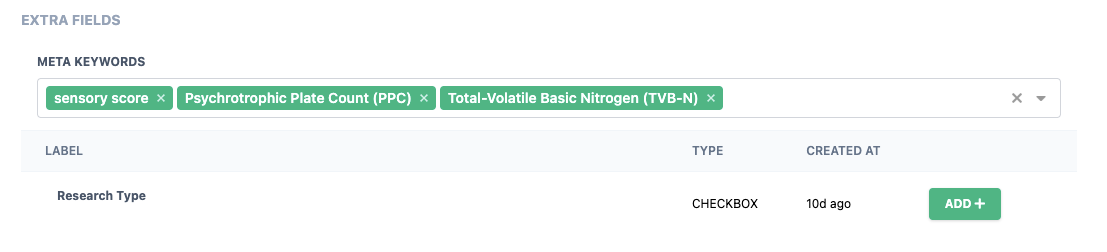
\includegraphics[width=1\textwidth]{slike/select_example_usage.png}
\end{center}
\caption{ Prikaz uporabe dinamično definiranega parametra, tipa $select$, z možnostjo izbere enega ali več podatkov }
\label{field-usage-example-select}
\end{figure}

Na sliki \ref{field-usage-example-select} je prikazana uporaba izbirnega polja. V tem primeru, lahko uporabnik izbere enega ali več podatkov za parameter \sn{Meta Keywords}. 

\subsection{Tipi podatkov}
Zaradi potrebe po razlikovanju po različnih tipov podatkov smo definirali več tipov ki predstavljajo podatek. Podatek predstavljen kot številka se ne odraža v sistem enako kot podatek, ki je predstavljen kot tekstovno polje. Katere vrse podatkov aplikacija podpira, je definirano v zalednem sistemu, in je dostopno preko aplikacijskega programskega vmestnika (glej kodo \ref{lst:supported-fields}). 

\begin{figure}[h]
    \centering
    \begin{lstlisting}[language=bash, style=mystyle,caption={Izsek aplikacijskega vmestinka za pridobitev vseh podprtih tipov v aplikaciji},label=lst:supported-fields]
curl --request GET \
  --url https://localhost:3001/api/fields/types \
  --header 'Authorization: Bearer ==token==' \
  --header 'Content-Type: application/json'
{
  "types": [
    {
      "name": "select",
      "has_values": true,
      "settings": [
        {
          "name": "string",
          "type": "number",
          "default_value": "string"
        }
      ]
    }
  ]
}
\end{lstlisting}
\end{figure}

\newpage
\subsubsection{Vnosno Polje}
Predstavlja podatek ki ga je potrebno vnesti vsakič znova in nima definirane nobene v naprej določene vrednosti. Vnosno polje je lahko predstavljeno kot številčna vrednost, ali pa kot tekstovno polje. 
Imamo možnost vnosa mnogih vrednosti za ta podatek, tako da definiramo podatek kot ponavljajoč podatek (\sn{repeatable}). To nam pride prav v primeru, kot je, če hočemo dodati zraven publikacije spletni vir, oziroma več njih.

\begin{figure}[h]
\begin{center}
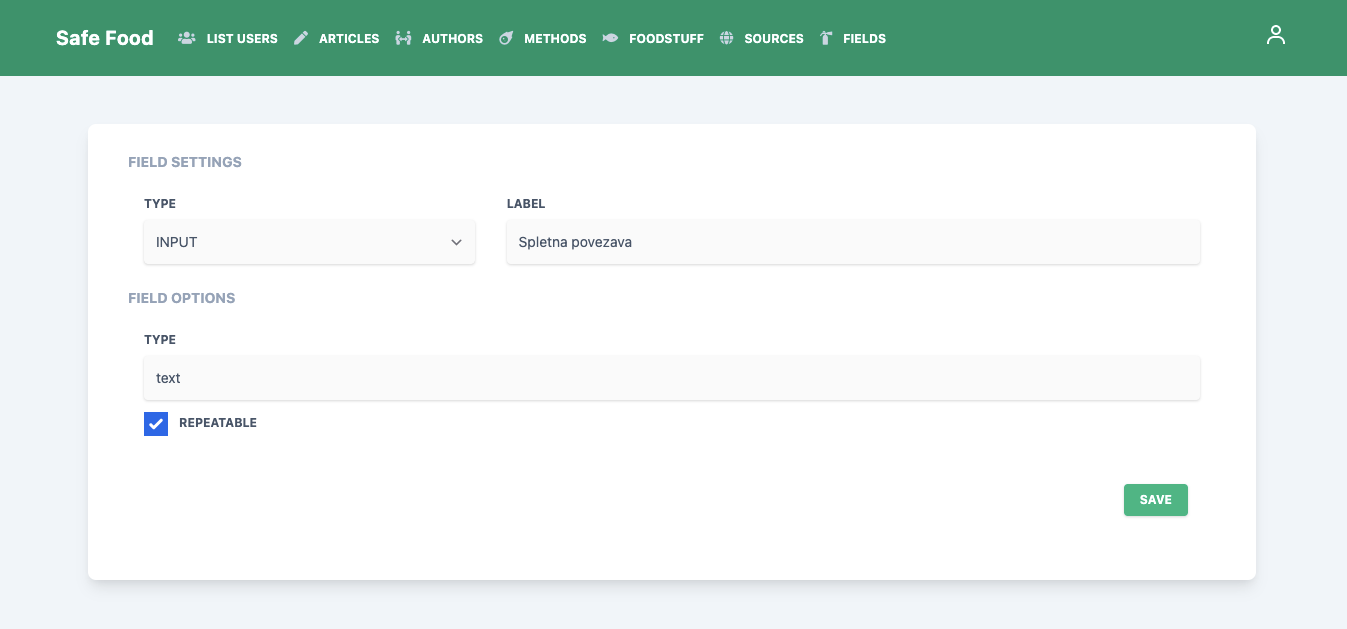
\includegraphics[width=1\textwidth]{slike/type_input.png}
\end{center}
\caption{ Definiranje vnosnega polja - input }
\label{type-input}
\end{figure}

Na sliki (\ref{type-input}) je razvidno, kako se definira podatek imenovan \sn{Spletna povezava}. Vrednost spletne povezava je tekstovnega tipa, zato smo za vrednost izbrali \verb=text=. Izbrali smo tudi vrednost \verb=repeatable=, ker želimo omogočiti več vnosov spletnih povezav. Dodan parameter se nam pojavi na voljo med urejanjem publikacije. 


Na dnu, se nam prikaže novo vnostno polje, katerega lahko izberemo in definiramo njegovo vrednost (glej sliko \ref{fields-usage}). Ker je parameter definiran, da je lahko predstavljen z več kot eno vrednostjo, se nam ponudi gumb za dodajanja nove vrednosti.

\begin{figure}[h]
\begin{center}
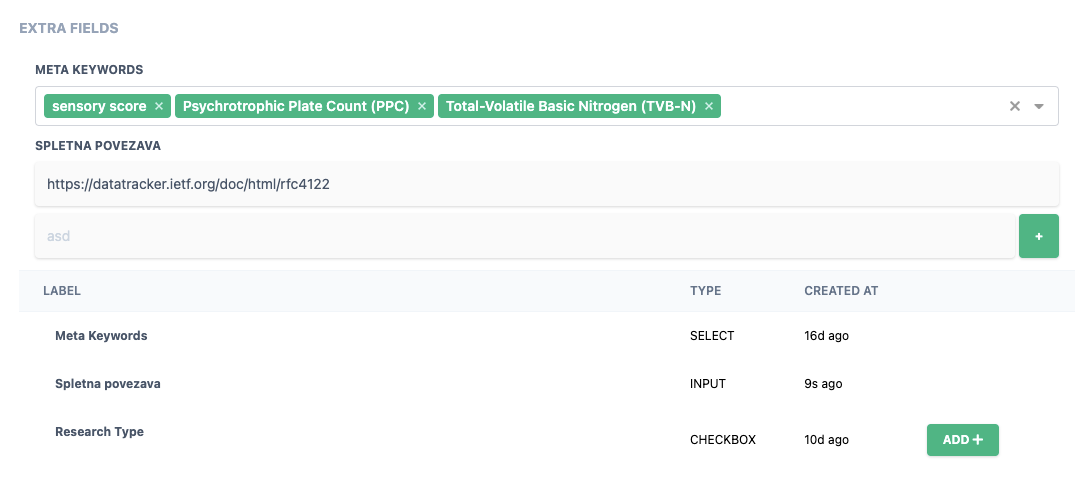
\includegraphics[width=1\textwidth]{slike/fields_usage.png}
\end{center}
\caption{ Prikaz uporabe dodanega parametra, med urejanjem publikacije }
\label{fields-usage}
\end{figure}


\subsubsection{Izbirno polje - Select}
\label{type-select-page}
Podatek predstavlja podobne vrednosti, kot vnostno polje \sn{Input} (\ref{type-input}), z razliko, da je so vrednosti lahko ze pred definirane. Pred definirane vrednosti omogočajo uporabniku hitrejše vnašanje podatkov. Na volje je tudi iskanje po vnešenih vrednostih in sprotno dodajanje le teh, v primeru, da vrednost še ne obstaja. Vse to je konfigurabilno, in se nastavi med samim definiranjem parametra (glej sliko \ref{type-select}. Na voljo je tudi možnost izbire več kot ene vrednosti, z izbiro opcije \sn{multiple} (prikazano na sliki \ref{fields-usage}). 


\begin{description}
\item[Opis posameznih opcij, med samim defineranjem parametra]:
	\begin{itemize}
		\item \textbf{taggable} - omogoča dodajanje novih vrednosti med samim urejanjem
		\item \textbf{multiple} - omogoča izbiro več kot ene vrednosti
		\item \textbf{searchable} - omogoča iskanje po vnesenih vrednostih
	\end{itemize}
\end{description}

\begin{figure}[H]
\begin{center}
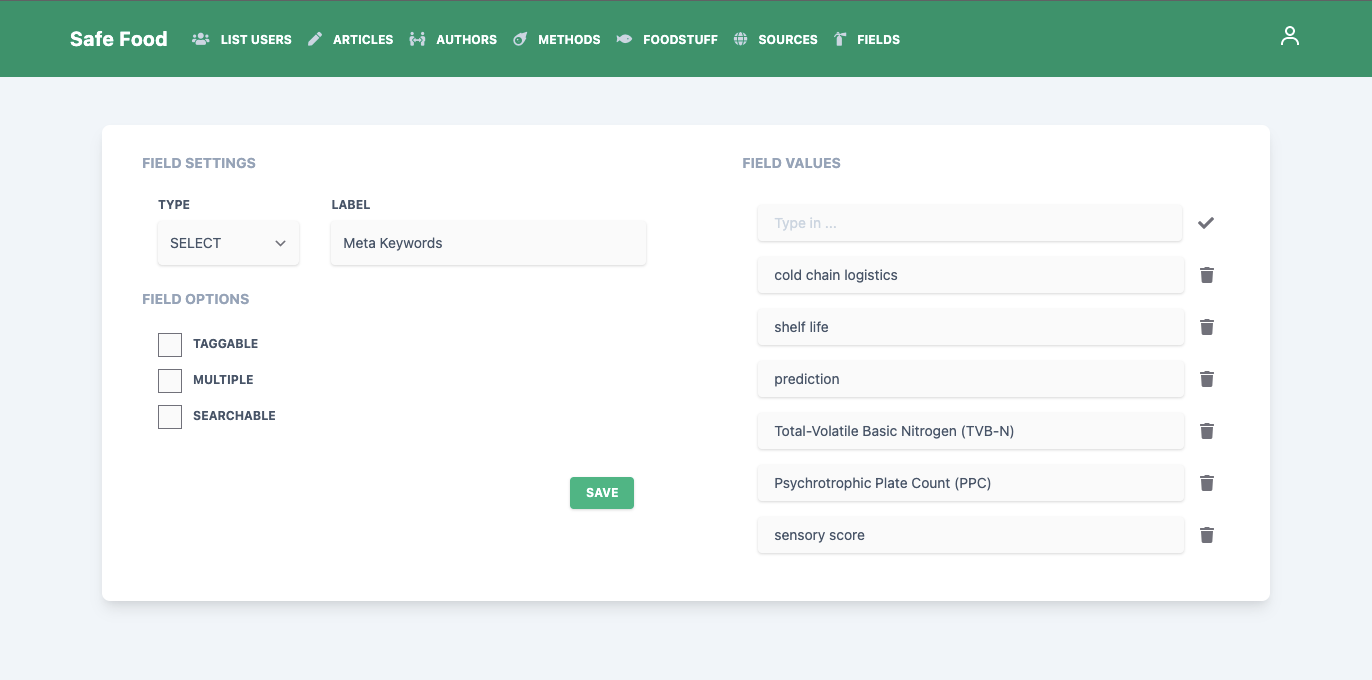
\includegraphics[width=1\textwidth]{slike/type_select.png}
\end{center}
\caption{ Definiranje vnosnega polja - select }
\label{type-select}
\end{figure}


\subsubsection{Izbirno polje - checkbox}
\label{type-checkbox-page}
Predstavlja podatek katere vrednosti so statične in pred definirane. Vnos podatkov je podoben kot pri \sn{Izbernem polju - Select} (\ref{type-select-page}), z razliko, da je podatek prikazan na drugačen način. Ta tip podatka nam ne omogoča iskanja po vrednostih in sprotnega dodajanja med samim urejanjem publikacije.

\begin{figure}[H]
\begin{center}
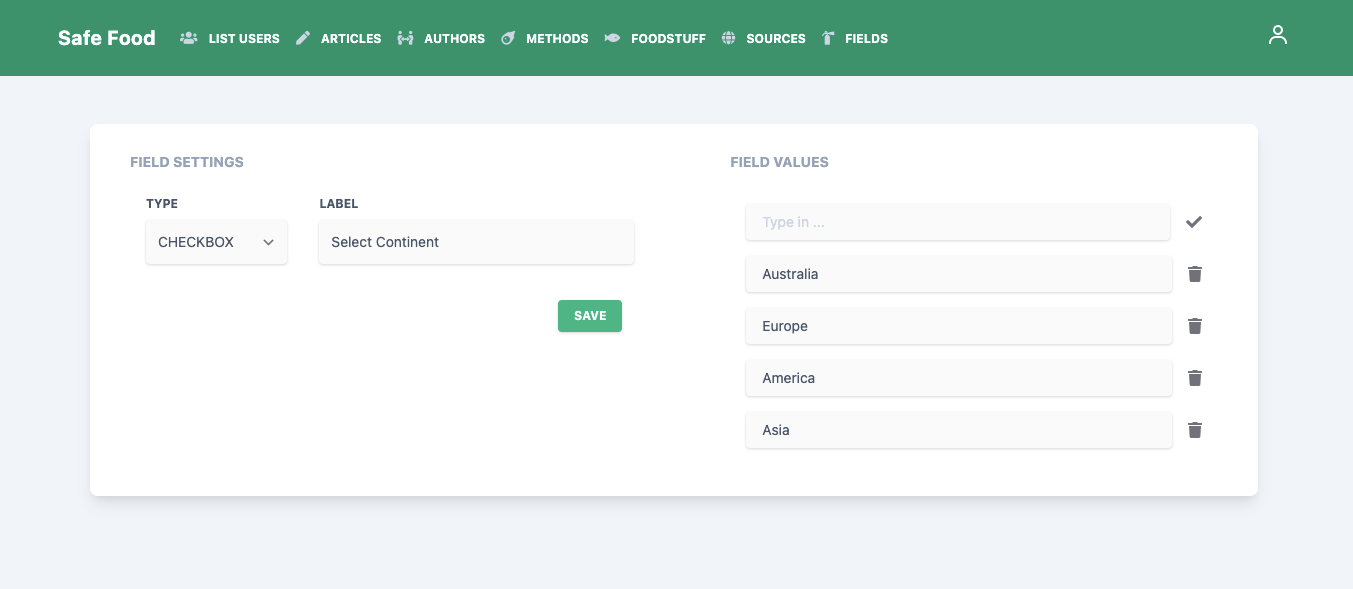
\includegraphics[width=1\textwidth]{slike/type_checkbox.png}
\end{center}
\caption{ Definiranje vnosnega polja - checkbox }
\label{type-checkbox}
\end{figure}


\subsubsection{Nalaganje datoteke}
Komponenta nam omogoča nalaganje datoteke za posamezno publicitacijo. Na voljo je dodajanje slik in datotek tipa \verb=".pdf"=, ostalih vrst datotek aplikacija ne sprejme.
\begin{figure}[h]
\begin{center}

\includegraphics[width=1\textwidth]{slike/upload_file_zone.png}

\includegraphics[width=1\textwidth]{slike/upload_file_list.png}
\end{center}
\caption{ Prikaz grafičnega vmestnika za nalaganje datotek }
\label{type-checkbox}
\end{figure}

\subsubsection{Polje za izbiranje časovnega podatka (datum)}
Predstavlja podatek, katera vrednost je časovna. Uporabniku je omogočeno definiranje podatka z izbiro datuma in časa na koledarju in časovnici (\ref{type-date}). 

Uporabili smo minimalistično knjižnico \verb=Day.js=, ki razčlenjuje, preverja, manipulira in prikazuje datume in ure za sodobne brskalnike z enostivnim aplikacijskim vmestnikom. Ponuja tudi podporo z ostalimi knjižnicami, kot je naprimer bolj prizna knjižnica \verb=Moment.js=.


\begin{figure}[h]
\begin{center}
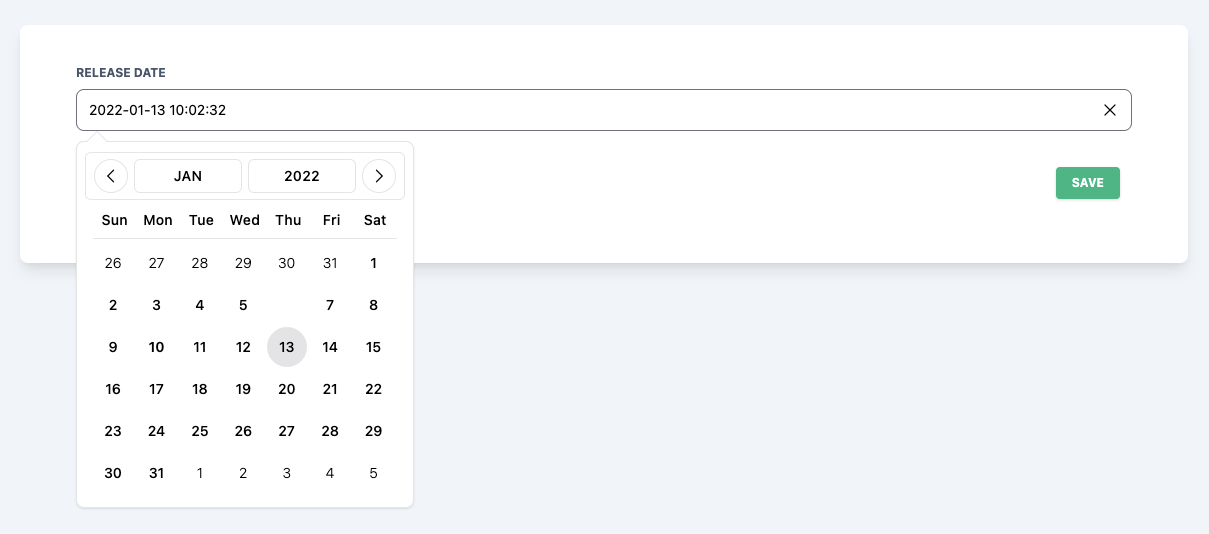
\includegraphics[width=1\textwidth]{slike/type_date.png}
\end{center}
\caption{ Prikaz grafičnega vmestnika za izbiranje datuma }
\label{type-date}
\end{figure}


\section{Vnos publikacije}
Uporabnik z pravicami urejanja ali dodajanja publikacij imajo dostop do strani \sn{Articles}. Na strani je prikazan seznam vseh vnesenih publikacij. Ker je vsako publikacijo mogoče urediti ali izbrisati, se na desni strani nahaja polje z ikonami, kjer je na voljo urejanje in brisanje posamezne publikacije. V primeru, da je vnesenih publikacij veliko, mora uporabnik uporabiti paginacijo na dnu strani, s katero se pomika med stranimi. Ima pa tudi možnost iskanja po naslovu publikacije. Seznam publikacij je prikazan z novejšimi publikacijami na vrhu (glej sliko \ref{list-articles}). Na strani se nahaja tudi gumb za dodajanje nove publikacije.

S klikom na ikono za urejanje se odpre stran z izpolnjenim spletnim obrazcom, s podatki o vnešeni publikaciji (glej sliko \ref{edit-articles}). V ozadju se uporablja ista \verb=vue.js= komponenta tudi za kreiranje nove publikacije. V primeru kreiranja nove publikacije, je potrebno ob shranjevanju poslati drugačen zahtevek kot v primeru urejanja. 

V primeru urejanja, se v URL naslovu nahaja identifikator publikacije, ki jo urejamo. Z uporabo tega identifikatorja pošljemo zahtevek na zaledni sistem, kjer dobimo vse potrebne informacije, ki so bile vnešene za dano publikacijo. Ob nalaganju spletnega obrazca moramo zagotoviti še ostale podatke kot so avtorji, metode, živila, viri, in dinamični podatki, katere je uporabnik definiral naknadno. Za vse te podatke imamo na voljo posamezne API vire, na katere pošljemo zahtevek za pridobitev teh podatkov. Na spletnem obrazcu je mogoče dodajati in urejati naslednje stvari:

\begin{description}
  \item \textbf{Datum objave} - datumsko polje, kdaj naj bo publikacija na voljo ostalim uporabnikom. Ta parameter je na voljo le administratorjem.
  \item \textbf{Vir} - izbirno polje za izbiro vira, na katerega se nanaša vnesena poublikacija. Z klikom na polje se nam odpre spusno okno, z prej vnešenimi viri. Imamo tudi možnost iskanja vira njegovem naslovu. V primeru da vir še ne obstaja, imamo na boljo gumb za dodajanje (+) novega vira. S klikom na gumb se nam odpre okno za kreiranje novega vira (glej sliko \ref{add-source}). Ob shranjevanju vira, se samodejno izpolne polje, z virom, ki je bil na novo vnešen.
  \item \textbf{Naslov} - tekstovno polje, ki predstavlja naslov publikacije
  \item \textbf{Leto} - numerično polje, ki predstavlja leto izdaje publikacije
  \item \textbf{Spletni vir} - predstavlja spletni vir, kjer lahko pridobimo več informacij o publikaciji
  \item \textbf{Avtorji} - izbirno polje za izbiro enega ali več avtorjev. Ob kliku na polje se nam odpre spustni meni z seznamom avtorjev, po katerih lahko izvajamo iskanje. V primeru, da avtor ne obstaja, imamo možnost dodajanja novega avtorja z pisanjem njegovega imena. Ob potrditvi, bo avtor avtomatsko kreiran v zalednem sistemu, in izbran v izbirnem polju (glej sliko \ref{multiselect}).
  \item \textbf{Metode} - uporablja se enaka komponenta kot pri polju za izbiro avtorjev, le da se v tem primeru izbirajo metode. 
  \item \textbf{Živila} - uporablja se enaka komponenta kot pri polju za izbiro avtorjev, le da se v tem primeru izbirajo živila.
  \item \textbf{Temperaturno območje} - predstavlja območje dveh števil, katerega je mogoče izbrati z horizontalnim drsnikom, ali pa z vpisom vrednosti v posamezna polja (minimalno in maksimalno vrednost).
  \item \textbf{Komentar} - tekstovno polje, kjer je mogoče vnesti daljše besedilo, do 255 znakov
  \item \textbf{Priponka} - polje za odlaganje datoteke. Na voljo nam je izbira datotek, katera je pripeta k publikaciji. Pripeta datoteka se prikaže znotraj komponente, in jo je mogoče odstraniti.
   \item \textbf{Dodatna polja} - seznam dodatnih polj, katere lahko dodatno definiramo. Na seznamu imamo možnost izbire dodatnega polja, ki ga želimo dodati k publikaciji. S klikom, se nam pojavi polje, za definiranje vrednost tega podatka. Vnosno polje se prikaže različno glede na tip podatka, ki ga izberemo.
\end{description}

S klikom na gumb \sn{Save}, ki se nahaja spodaj desno, sprožimo zahtevek za shranjevanje vnesenih podatkov. V primeru, da podatki niso bili pravilno nastavljeni se na obrazcu poleg posameznih polj pojavijo napake, z opisom kaj je narobe. Ob uspešnem shranjevanju se pokaže sporočilo, da je bila publikacija uspešno shranjena. 

\begin{figure}[h]
\begin{center}
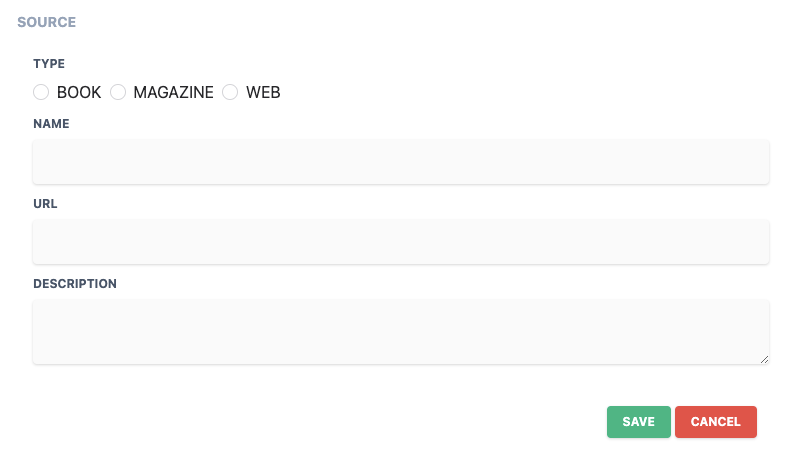
\includegraphics[width=0.75\textwidth]{slike/add-source.png}
\end{center}
\caption{ Obrazec za dodajanje novega vira }
\label{add-source}
\end{figure}


\begin{figure}[h]
\begin{center}

\includegraphics[width=0.5\textwidth]{slike/multiselect.png}
\end{center}
\caption{ Spustni meni z predlaganimi vrednostmi }
\label{multiselect}
\end{figure}

\begin{figure}[h]
\begin{center}
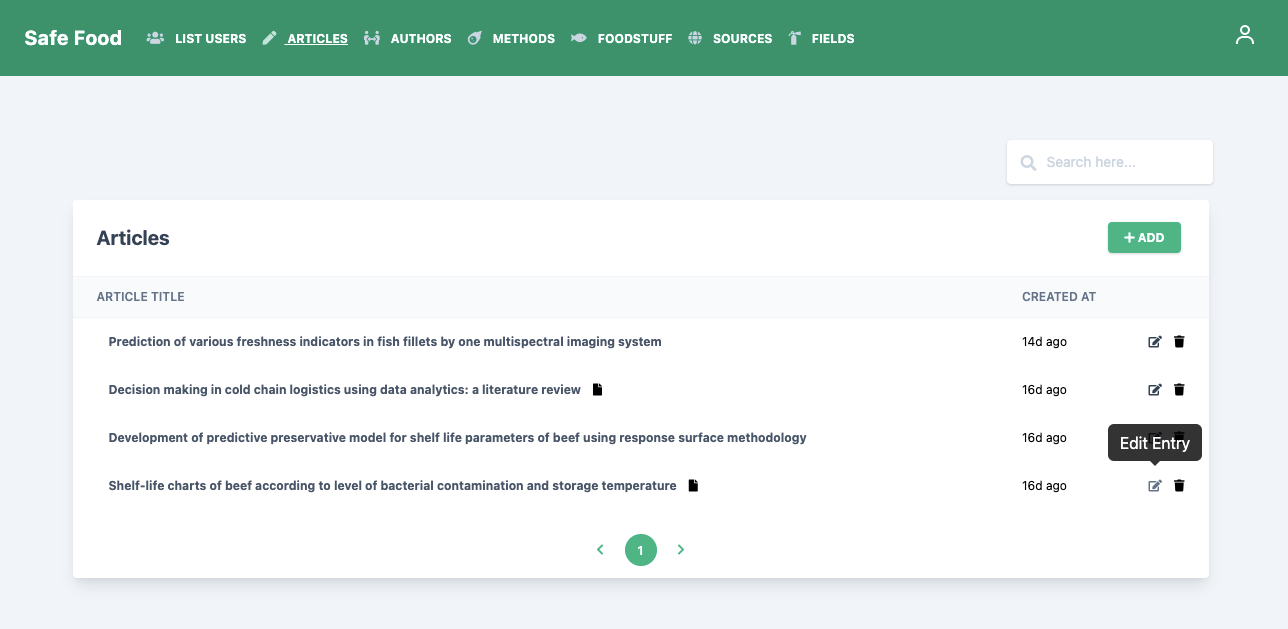
\includegraphics[width=1\textwidth]{slike/list-articles.png}
\end{center}
\caption{ Seznam publikacij v administraciji }
\label{list-articles}
\end{figure}


\begin{figure}[h]
\begin{center}
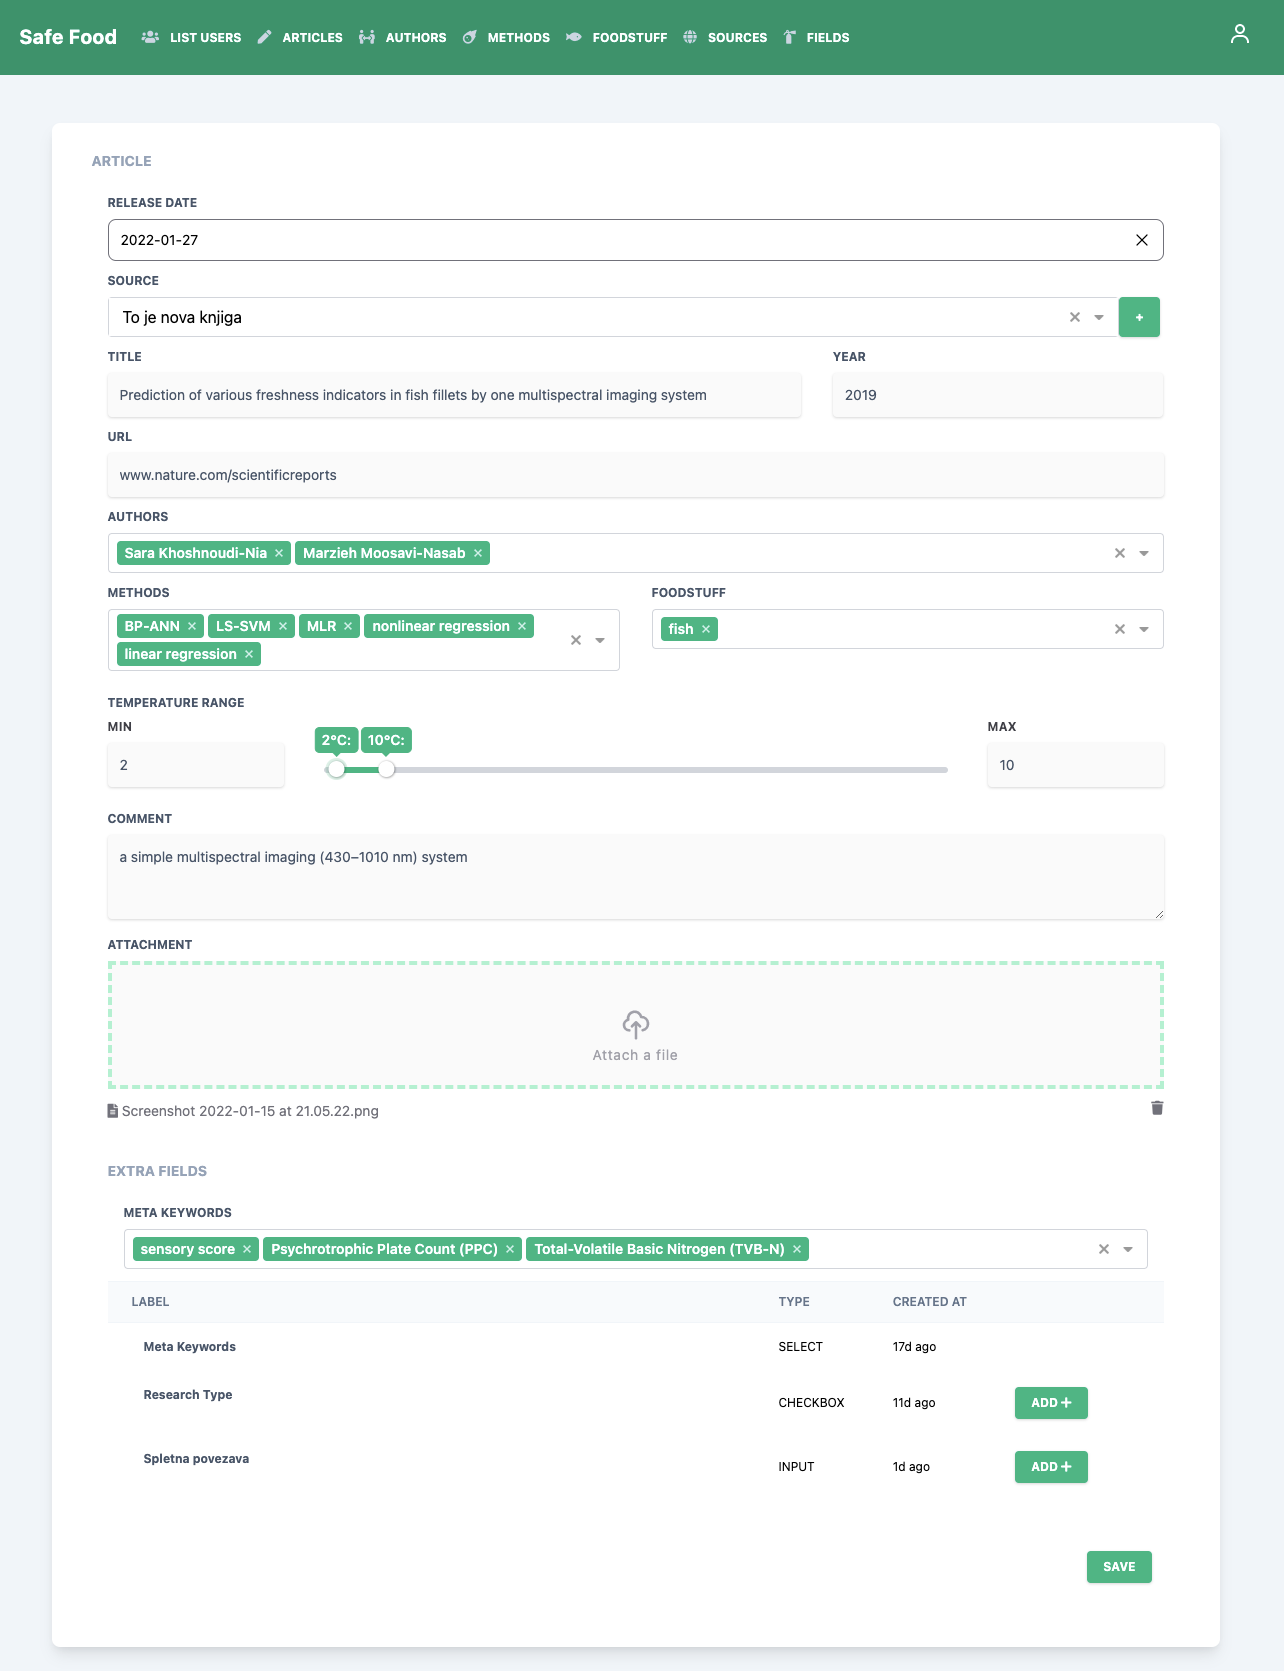
\includegraphics[width=1\textwidth]{slike/form-create-article.png}
\end{center}
\caption{ Spletni obrazec za urejanje ali vnos nove publikacije }
\label{edit-articles}
\end{figure}

\clearpage
\section{Iskanje publikacij}
\label{filters-page}
Vse vnešene publikacije so uporabniku prijazno prikazane na eni strani. Uporabnik ima možnost uporabe številnih filtrov, in s tem hitreje najde publikacijo, ki jo išče. Iskanje je omogočeno po vseh možnih podatkih, vnesenih za posamezno publikacijo. 

Stran je razdeljena na dva dela. Na levem delu strani so uporabniku na voljo filtri, katere lahko uporabi za iskanje po publikacijah, na desnem delu strani pa se uporabiku te publikacije prikažejo. 

Uporaba filtrov je enostavna. Na levem delu so izpisani vsi podatki, po katerih je mogoče iskati. Ob kliku na filter, se prikaže nabor vrednosti, katere lahko uporabik izbera, in s tem vklopi ali izklopi filter. V zgornjem delu strani je na voljo tudi iskanje po tekstovnem nizu besed, kjer uporabnik vnese iskan niz, in glede na niz se izvede filtracija. 


Na sliki \ref{seach example} je prikazana praktična uporaba filtrov. V kombinaciji filtrov smo dobili rezultat, ki upošteva vse naštete filtre. 

\begin{figure}[h]
\begin{center}

\includegraphics[width=1\textwidth]{slike/search.png}
\end{center}
\caption{ Prikaz uporabe filtrov }
\label{seach example}
\end{figure}




\chapter{Sklepne ugotovitve}
Nadaljni razvoj aplikacije bi lahko potekal v smeri brezglavega urejevalnika vsebin, kar pomeni, da bi zasnovali aplikacijski vmestnih za dinamično urejanje podatkov. Zaradi arhitekturne zasnove je enostavno izluščiti del dinamičnega dodajanja podatkov. S tem bi naredili novo mikrostoritev, ki bi skrbela za definiranje, shranjevanje, urejanje in brisanje dinamičnih podatkov. 

S tem bi imeli rešitev za različne vrste podatkov, ne samo za naš trenutni primer, za vnašanje razikovalnih metod. 


% \newpage %dodaj po potrebi, da bo številka strani za Literaturo v Kazalu pravilna!
% \\
\clearpage
\addcontentsline{toc}{chapter}{Literatura}
\bibliographystyle{plain}
\bibliography{diploma}


\end{document}

